\documentclass[]{article}
\usepackage{lmodern}
\usepackage{amssymb,amsmath}
\usepackage{ifxetex,ifluatex}
\usepackage{fixltx2e} % provides \textsubscript
\ifnum 0\ifxetex 1\fi\ifluatex 1\fi=0 % if pdftex
  \usepackage[T1]{fontenc}
  \usepackage[utf8]{inputenc}
\else % if luatex or xelatex
  \ifxetex
    \usepackage{mathspec}
  \else
    \usepackage{fontspec}
  \fi
  \defaultfontfeatures{Ligatures=TeX,Scale=MatchLowercase}
\fi
% use upquote if available, for straight quotes in verbatim environments
\IfFileExists{upquote.sty}{\usepackage{upquote}}{}
% use microtype if available
\IfFileExists{microtype.sty}{%
\usepackage{microtype}
\UseMicrotypeSet[protrusion]{basicmath} % disable protrusion for tt fonts
}{}
\usepackage[margin=1in]{geometry}
\usepackage{hyperref}
\hypersetup{unicode=true,
            pdftitle={ChIP-seq Analysis of TGF-beta Treated SMAD2 and SMAD3 Peaks},
            pdfborder={0 0 0},
            breaklinks=true}
\urlstyle{same}  % don't use monospace font for urls
\usepackage{color}
\usepackage{fancyvrb}
\newcommand{\VerbBar}{|}
\newcommand{\VERB}{\Verb[commandchars=\\\{\}]}
\DefineVerbatimEnvironment{Highlighting}{Verbatim}{commandchars=\\\{\}}
% Add ',fontsize=\small' for more characters per line
\usepackage{framed}
\definecolor{shadecolor}{RGB}{248,248,248}
\newenvironment{Shaded}{\begin{snugshade}}{\end{snugshade}}
\newcommand{\AlertTok}[1]{\textcolor[rgb]{0.94,0.16,0.16}{#1}}
\newcommand{\AnnotationTok}[1]{\textcolor[rgb]{0.56,0.35,0.01}{\textbf{\textit{#1}}}}
\newcommand{\AttributeTok}[1]{\textcolor[rgb]{0.77,0.63,0.00}{#1}}
\newcommand{\BaseNTok}[1]{\textcolor[rgb]{0.00,0.00,0.81}{#1}}
\newcommand{\BuiltInTok}[1]{#1}
\newcommand{\CharTok}[1]{\textcolor[rgb]{0.31,0.60,0.02}{#1}}
\newcommand{\CommentTok}[1]{\textcolor[rgb]{0.56,0.35,0.01}{\textit{#1}}}
\newcommand{\CommentVarTok}[1]{\textcolor[rgb]{0.56,0.35,0.01}{\textbf{\textit{#1}}}}
\newcommand{\ConstantTok}[1]{\textcolor[rgb]{0.00,0.00,0.00}{#1}}
\newcommand{\ControlFlowTok}[1]{\textcolor[rgb]{0.13,0.29,0.53}{\textbf{#1}}}
\newcommand{\DataTypeTok}[1]{\textcolor[rgb]{0.13,0.29,0.53}{#1}}
\newcommand{\DecValTok}[1]{\textcolor[rgb]{0.00,0.00,0.81}{#1}}
\newcommand{\DocumentationTok}[1]{\textcolor[rgb]{0.56,0.35,0.01}{\textbf{\textit{#1}}}}
\newcommand{\ErrorTok}[1]{\textcolor[rgb]{0.64,0.00,0.00}{\textbf{#1}}}
\newcommand{\ExtensionTok}[1]{#1}
\newcommand{\FloatTok}[1]{\textcolor[rgb]{0.00,0.00,0.81}{#1}}
\newcommand{\FunctionTok}[1]{\textcolor[rgb]{0.00,0.00,0.00}{#1}}
\newcommand{\ImportTok}[1]{#1}
\newcommand{\InformationTok}[1]{\textcolor[rgb]{0.56,0.35,0.01}{\textbf{\textit{#1}}}}
\newcommand{\KeywordTok}[1]{\textcolor[rgb]{0.13,0.29,0.53}{\textbf{#1}}}
\newcommand{\NormalTok}[1]{#1}
\newcommand{\OperatorTok}[1]{\textcolor[rgb]{0.81,0.36,0.00}{\textbf{#1}}}
\newcommand{\OtherTok}[1]{\textcolor[rgb]{0.56,0.35,0.01}{#1}}
\newcommand{\PreprocessorTok}[1]{\textcolor[rgb]{0.56,0.35,0.01}{\textit{#1}}}
\newcommand{\RegionMarkerTok}[1]{#1}
\newcommand{\SpecialCharTok}[1]{\textcolor[rgb]{0.00,0.00,0.00}{#1}}
\newcommand{\SpecialStringTok}[1]{\textcolor[rgb]{0.31,0.60,0.02}{#1}}
\newcommand{\StringTok}[1]{\textcolor[rgb]{0.31,0.60,0.02}{#1}}
\newcommand{\VariableTok}[1]{\textcolor[rgb]{0.00,0.00,0.00}{#1}}
\newcommand{\VerbatimStringTok}[1]{\textcolor[rgb]{0.31,0.60,0.02}{#1}}
\newcommand{\WarningTok}[1]{\textcolor[rgb]{0.56,0.35,0.01}{\textbf{\textit{#1}}}}
\usepackage{graphicx,grffile}
\makeatletter
\def\maxwidth{\ifdim\Gin@nat@width>\linewidth\linewidth\else\Gin@nat@width\fi}
\def\maxheight{\ifdim\Gin@nat@height>\textheight\textheight\else\Gin@nat@height\fi}
\makeatother
% Scale images if necessary, so that they will not overflow the page
% margins by default, and it is still possible to overwrite the defaults
% using explicit options in \includegraphics[width, height, ...]{}
\setkeys{Gin}{width=\maxwidth,height=\maxheight,keepaspectratio}
\IfFileExists{parskip.sty}{%
\usepackage{parskip}
}{% else
\setlength{\parindent}{0pt}
\setlength{\parskip}{6pt plus 2pt minus 1pt}
}
\setlength{\emergencystretch}{3em}  % prevent overfull lines
\providecommand{\tightlist}{%
  \setlength{\itemsep}{0pt}\setlength{\parskip}{0pt}}
\setcounter{secnumdepth}{0}
% Redefines (sub)paragraphs to behave more like sections
\ifx\paragraph\undefined\else
\let\oldparagraph\paragraph
\renewcommand{\paragraph}[1]{\oldparagraph{#1}\mbox{}}
\fi
\ifx\subparagraph\undefined\else
\let\oldsubparagraph\subparagraph
\renewcommand{\subparagraph}[1]{\oldsubparagraph{#1}\mbox{}}
\fi

%%% Use protect on footnotes to avoid problems with footnotes in titles
\let\rmarkdownfootnote\footnote%
\def\footnote{\protect\rmarkdownfootnote}

%%% Change title format to be more compact
\usepackage{titling}

% Create subtitle command for use in maketitle
\newcommand{\subtitle}[1]{
  \posttitle{
    \begin{center}\large#1\end{center}
    }
}

\setlength{\droptitle}{-2em}

  \title{ChIP-seq Analysis of TGF-beta Treated SMAD2 and SMAD3 Peaks}
    \pretitle{\vspace{\droptitle}\centering\huge}
  \posttitle{\par}
    \author{}
    \preauthor{}\postauthor{}
    \date{}
    \predate{}\postdate{}
  
\usepackage{booktabs}
\usepackage{longtable}
\usepackage{array}
\usepackage{multirow}
\usepackage{wrapfig}
\usepackage{float}
\usepackage{colortbl}
\usepackage{pdflscape}
\usepackage{tabu}
\usepackage{threeparttable}
\usepackage{threeparttablex}
\usepackage[normalem]{ulem}
\usepackage{makecell}
\usepackage{xcolor}

\begin{document}
\maketitle

\clearpage{}

\tableofcontents

\clearpage{}


\section{Methods and Code}

\textbf{Note:} the following code takes a long time to run. Hence, it
shall just be displayed here for transparency but will not be run to
compile the document.

Instead, the objects from the image saved in
``annotation\textunderscore go\textunderscore rough\textunderscore code.RData''
after running this code will be loaded to present and discuss the
results.


\subsection{Libraries}

The following libraries were loaded during this analysis:

\begin{enumerate}
\def\labelenumi{\arabic{enumi}.}
\item
  tidyverse
\item
  formatR
\item
  GenomicRanges
\item
  org.Hs.eg.db
\item
  TxDb.Hsapiens.UCSC.hg38.knownGene
\item
  ChIPseeker
\item
  clusterProfiler
\item
  kableExtra
\end{enumerate}

\textbf{Note:} Since the code takes a long time to run, the following
file which contains the results of the analyses carried out by code will
be loaded first, and the code will be displayed for transparency
purposes, but will not be evaluated.

\begin{Shaded}
\begin{Highlighting}[]
\KeywordTok{load}\NormalTok{(}\StringTok{"annotation_go_rough_code.RData"}\NormalTok{)}
\end{Highlighting}
\end{Shaded}


\subsection{Annotating Peaks}

Peaks were annotated using the \textbf{ChIPseeker} package. The
annotated peaks for each of the conditions were further filtered into
three subsets:

\begin{enumerate}
\def\labelenumi{\arabic{enumi}.}
\item
  All peaks
\item
  Peaks with only promoter annotations.
\item
  Peaks lying within genic regions, i.e., peaks without the annotations
  ``Distal Intergenic'' and ``Downstream''
\end{enumerate}

The following code was used to read in the file names and create a
character vector from them. Those names were then fed into a function to
convert those files into Granges objects held in a list.

\begin{Shaded}
\begin{Highlighting}[]
\NormalTok{knitr}\OperatorTok{::}\NormalTok{opts_chunk}\OperatorTok{$}\KeywordTok{set}\NormalTok{(}\DataTypeTok{echo =} \OtherTok{FALSE}\NormalTok{, }\DataTypeTok{tidy =} \OtherTok{TRUE}\NormalTok{)}

\CommentTok{## Takes a filename as string input, and if it has suffix '.narrowPeak',}
\CommentTok{## converts it to a GRanges object containing a q_value metadata column.}
\CommentTok{## Requires tidyverse and GRanges packages.}

\CommentTok{## checking for existence of file and correct extension}
\NormalTok{narrow_to_granges <-}\StringTok{ }\ControlFlowTok{function}\NormalTok{(file) \{}
    \KeywordTok{stopifnot}\NormalTok{(}\KeywordTok{file.exists}\NormalTok{(file), }\KeywordTok{endsWith}\NormalTok{(}\DataTypeTok{x =}\NormalTok{ file, }\DataTypeTok{suffix =} \StringTok{".narrowPeak"}\NormalTok{))}
    
    
\NormalTok{    bed <-}\StringTok{ }\KeywordTok{as_tibble}\NormalTok{(}\KeywordTok{read_tsv}\NormalTok{(}\DataTypeTok{file =}\NormalTok{ file, }\DataTypeTok{col_names =} \KeywordTok{c}\NormalTok{(}\StringTok{"chrom"}\NormalTok{, }\StringTok{"start"}\NormalTok{, }\StringTok{"end"}\NormalTok{, }
        \StringTok{"name"}\NormalTok{, }\StringTok{"score"}\NormalTok{, }\StringTok{"strand"}\NormalTok{, }\StringTok{"signal_value"}\NormalTok{, }\StringTok{"p_value"}\NormalTok{, }\StringTok{"q_value"}\NormalTok{, }\StringTok{"peak"}\NormalTok{)))}
    
    
\NormalTok{    gr <-}\StringTok{ }\KeywordTok{GRanges}\NormalTok{(}\DataTypeTok{seqnames =}\NormalTok{ bed}\OperatorTok{$}\NormalTok{chrom, }\DataTypeTok{ranges =} \KeywordTok{IRanges}\NormalTok{(}\DataTypeTok{start =}\NormalTok{ bed}\OperatorTok{$}\NormalTok{start, }
        \DataTypeTok{end =}\NormalTok{ bed}\OperatorTok{$}\NormalTok{end), }\DataTypeTok{strand =} \KeywordTok{if_else}\NormalTok{(}\DataTypeTok{condition =}\NormalTok{ bed}\OperatorTok{$}\NormalTok{strand }\OperatorTok{==}\StringTok{ "+"} \OperatorTok{|}\StringTok{ }\NormalTok{bed}\OperatorTok{$}\NormalTok{strand }\OperatorTok{==}\StringTok{ }
\StringTok{        "-"}\NormalTok{, }\DataTypeTok{true =}\NormalTok{ bed}\OperatorTok{$}\NormalTok{strand, }\DataTypeTok{false =} \StringTok{"*"}\NormalTok{), }\DataTypeTok{q_value =}\NormalTok{ bed}\OperatorTok{$}\NormalTok{q_value)}
    
    \KeywordTok{return}\NormalTok{(gr)}
\NormalTok{\}}


\CommentTok{### To read in multiple .narrowPeak files and create a GRanges list of GRanges}
\CommentTok{### objects with the input of respective files.}

\NormalTok{files <-}\StringTok{ }\KeywordTok{dir}\NormalTok{(}\DataTypeTok{path =} \StringTok{"."}\NormalTok{, }\DataTypeTok{pattern =} \StringTok{"}\CharTok{\textbackslash{}\textbackslash{}}\StringTok{.narrowPeak$"}\NormalTok{)  }\CommentTok{## specify files in character vector}

\NormalTok{grl <-}\StringTok{ }\KeywordTok{lapply}\NormalTok{(files, narrow_to_granges)  }\CommentTok{## Create list of GRanges object}
\end{Highlighting}
\end{Shaded}

Here are the contents of the files vector.

\begin{Shaded}
\begin{Highlighting}[]
\NormalTok{files}
\end{Highlighting}
\end{Shaded}

\begin{verbatim}
## [1] "SMAD2_abInput_treated_peaks.narrowPeak"  
## [2] "SMAD2_abInput_untreated_peaks.narrowPeak"
## [3] "SMAD3_LAP_treated_peaks.narrowPeak"      
## [4] "SMAD3_LAP_untreated_peaks.narrowPeak"
\end{verbatim}

The following code was then used to assign the Granges in the list to
separate variables. The name of the variable to hold each GRange object
was derived from the respective file name from which its data was
obtained. The names of the variables were stored as a character vector
``v''.To names in v, the respective GRange was assigned.

\begin{Shaded}
\begin{Highlighting}[]
\NormalTok{TxDb <-}\StringTok{ }\NormalTok{TxDb.Hsapiens.UCSC.hg38.knownGene}

\CommentTok{## vector of variable names for granges in list}

\NormalTok{v <-}\StringTok{ }\KeywordTok{str_remove_all}\NormalTok{(}\DataTypeTok{string =}\NormalTok{ files, }\DataTypeTok{pattern =} \StringTok{"}\CharTok{\textbackslash{}\textbackslash{}}\StringTok{.narrowPeak$"}\NormalTok{)}

\CommentTok{### Assign individual granges within grl to variable names in v.}

\ControlFlowTok{for}\NormalTok{ (i }\ControlFlowTok{in} \KeywordTok{seq_along}\NormalTok{(grl)) \{}
    \KeywordTok{assign}\NormalTok{(}\DataTypeTok{x =}\NormalTok{ v[i], }\DataTypeTok{value =}\NormalTok{ grl[[i]])}
\NormalTok{\}}
\end{Highlighting}
\end{Shaded}

Here are the names of the variables held in vector v:

\begin{Shaded}
\begin{Highlighting}[]
\NormalTok{v}
\end{Highlighting}
\end{Shaded}

\begin{verbatim}
## [1] "SMAD2_abInput_treated_peaks"   "SMAD2_abInput_untreated_peaks"
## [3] "SMAD3_LAP_treated_peaks"       "SMAD3_LAP_untreated_peaks"
\end{verbatim}

A character vector of variable names was created to hold the annotated
peak objects derived from the GRanges.

\begin{Shaded}
\begin{Highlighting}[]
\NormalTok{ap_v <-}\StringTok{ }\KeywordTok{paste0}\NormalTok{(}\StringTok{"AP_"}\NormalTok{, v)  }\CommentTok{## variable names for annotated peak objects}


\CommentTok{### Create annotated peak objects and assign them to names in ap_v}

\ControlFlowTok{for}\NormalTok{ (i }\ControlFlowTok{in} \KeywordTok{seq_along}\NormalTok{(grl)) \{}
    \KeywordTok{assign}\NormalTok{(}\DataTypeTok{x =}\NormalTok{ ap_v[i], }\DataTypeTok{value =} \KeywordTok{annotatePeak}\NormalTok{(}\DataTypeTok{peak =}\NormalTok{ grl[[i]], }\DataTypeTok{TxDb =}\NormalTok{ TxDb, }\DataTypeTok{annoDb =} \StringTok{"org.Hs.eg.db"}\NormalTok{))}
\NormalTok{\}}


\NormalTok{df_ap_v <-}\StringTok{ }\KeywordTok{paste0}\NormalTok{(}\StringTok{"df_"}\NormalTok{, ap_v)  }\CommentTok{## variable names for tibbles derived from annotated peaks}


\CommentTok{### Create tibbles from annotated peak objects listed in ap_v and assign them}
\CommentTok{### to names in df_ap_v}

\ControlFlowTok{for}\NormalTok{ (i }\ControlFlowTok{in} \KeywordTok{seq_along}\NormalTok{(ap_v)) \{}
    \KeywordTok{assign}\NormalTok{(}\DataTypeTok{x =}\NormalTok{ df_ap_v[i], }\DataTypeTok{value =} \KeywordTok{parse}\NormalTok{(}\DataTypeTok{text =}\NormalTok{ ap_v[i]) }\OperatorTok\StringTok{ }\KeywordTok{eval}\NormalTok{() }\OperatorTok\StringTok{ }\NormalTok{AnnotationDbi}\OperatorTok{::}\KeywordTok{as.data.frame}\NormalTok{() }\OperatorTok\StringTok{ }
\StringTok{        }\KeywordTok{as_tibble}\NormalTok{())}
\NormalTok{\}}

\CommentTok{## variable names for tibbles derived from annotated peaks limited to}
\CommentTok{## promoter annotations}

\NormalTok{prom_df_ap_v <-}\StringTok{ }\KeywordTok{paste0}\NormalTok{(}\StringTok{"prom_df_"}\NormalTok{, ap_v)}


\CommentTok{### Create subset of tibbles from variable names listed in df_ap_v and assign}
\CommentTok{### them to variable names in prom_df_ap_v}
\ControlFlowTok{for}\NormalTok{ (i }\ControlFlowTok{in} \KeywordTok{seq_along}\NormalTok{(df_ap_v)) \{}
    \KeywordTok{assign}\NormalTok{(}\DataTypeTok{x =}\NormalTok{ prom_df_ap_v[i], }\DataTypeTok{value =} \KeywordTok{parse}\NormalTok{(}\DataTypeTok{text =}\NormalTok{ df_ap_v[i]) }\OperatorTok\StringTok{ }\KeywordTok{eval}\NormalTok{() }\OperatorTok\StringTok{ }
\StringTok{        }\KeywordTok{filter}\NormalTok{(}\KeywordTok{str_detect}\NormalTok{(annotation, }\StringTok{"Promoter"}\NormalTok{)))}
\NormalTok{\}}

\CommentTok{## variable names for tibbles derived from annotated peaks limited to gene}
\CommentTok{## region annotations}

\NormalTok{gen_df_ap_v <-}\StringTok{ }\KeywordTok{paste0}\NormalTok{(}\StringTok{"gen_df_"}\NormalTok{, ap_v)}


\CommentTok{### Filter tibbles with variable names listed in df_ap_v to discard rows with}
\CommentTok{### 'Distal Intergenic' or 'Downstream' annotations and assign them to names}
\CommentTok{### in gen_df_ap_v.}

\ControlFlowTok{for}\NormalTok{ (i }\ControlFlowTok{in} \KeywordTok{seq_along}\NormalTok{(df_ap_v)) \{}
    \KeywordTok{assign}\NormalTok{(}\DataTypeTok{x =}\NormalTok{ gen_df_ap_v[i], }\DataTypeTok{value =} \KeywordTok{parse}\NormalTok{(}\DataTypeTok{text =}\NormalTok{ df_ap_v[i]) }\OperatorTok\StringTok{ }\KeywordTok{eval}\NormalTok{() }\OperatorTok\StringTok{ }
\StringTok{        }\KeywordTok{filter}\NormalTok{(}\OperatorTok{!}\KeywordTok{str_detect}\NormalTok{(annotation, }\StringTok{"Distal Intergenic|Downstream"}\NormalTok{)))}
\NormalTok{\}}
\end{Highlighting}
\end{Shaded}


\subsection{GO Term Enrichment Analysis of Annotated Peaks}

GO term enrichment analysis of the annotated peaks was carried out using
the \textbf{ClusterProfiler} package. Analysis was carried out for all
four conditions and each subset of annotated peaks within each condition
(all peaks, promoter-limited peaks and genic region-limited peaks).

\textbf{Note:} The following code takes \emph{very} long to run.

\begin{Shaded}
\begin{Highlighting}[]
\NormalTok{ego_v <-}\StringTok{ }\KeywordTok{paste0}\NormalTok{(}\StringTok{"ego_"}\NormalTok{, v)  }\CommentTok{### Vector of variable names for go term enrichment objects}



\ControlFlowTok{for}\NormalTok{ (i }\ControlFlowTok{in} \KeywordTok{seq_along}\NormalTok{(ego_v)) \{}
\NormalTok{    ego <-}\StringTok{ }\KeywordTok{parse}\NormalTok{(}\DataTypeTok{text =}\NormalTok{ df_ap_v[i]) }\OperatorTok\StringTok{ }\KeywordTok{eval}\NormalTok{(}\DataTypeTok{expr =}\NormalTok{ .) }\OperatorTok\StringTok{ }\NormalTok{dplyr}\OperatorTok{::}\KeywordTok{select}\NormalTok{(geneId) }\OperatorTok\StringTok{ }
\StringTok{        }\KeywordTok{unlist}\NormalTok{() }\OperatorTok\StringTok{ }\KeywordTok{enrichGO}\NormalTok{(}\DataTypeTok{gene =}\NormalTok{ ., }\DataTypeTok{OrgDb =}\NormalTok{ org.Hs.eg.db, }\DataTypeTok{ont =} \StringTok{"BP"}\NormalTok{, }\DataTypeTok{pAdjustMethod =} \StringTok{"BH"}\NormalTok{, }
        \DataTypeTok{readable =} \OtherTok{TRUE}\NormalTok{)}
    \ControlFlowTok{if}\NormalTok{ (}\OperatorTok{!}\KeywordTok{nrow}\NormalTok{(}\KeywordTok{as.data.frame}\NormalTok{(ego)) }\OperatorTok{==}\StringTok{ }\DecValTok{0}\NormalTok{) }
        \KeywordTok{assign}\NormalTok{(}\DataTypeTok{x =}\NormalTok{ ego_v[i], }\DataTypeTok{value =}\NormalTok{ ego)}
\NormalTok{\}}



\CommentTok{### Vector of variable names for go term enrichment objects limited to}
\CommentTok{### promoter peaks}

\NormalTok{prom_ego_v <-}\StringTok{ }\NormalTok{ego_v <-}\StringTok{ }\KeywordTok{paste0}\NormalTok{(}\StringTok{"prom_ego_"}\NormalTok{, v)}

\CommentTok{### Performing go term analysis using the clusterprofiler package and}
\CommentTok{### assigning the results to the variables in gen_ego_v}

\ControlFlowTok{for}\NormalTok{ (i }\ControlFlowTok{in} \KeywordTok{seq_along}\NormalTok{(prom_ego_v)) \{}
\NormalTok{    ego <-}\StringTok{ }\KeywordTok{parse}\NormalTok{(}\DataTypeTok{text =}\NormalTok{ prom_df_ap_v[i]) }\OperatorTok\StringTok{ }\KeywordTok{eval}\NormalTok{(}\DataTypeTok{expr =}\NormalTok{ .) }\OperatorTok\StringTok{ }\NormalTok{dplyr}\OperatorTok{::}\KeywordTok{select}\NormalTok{(geneId) }\OperatorTok\StringTok{ }
\StringTok{        }\KeywordTok{unlist}\NormalTok{() }\OperatorTok\StringTok{ }\KeywordTok{enrichGO}\NormalTok{(}\DataTypeTok{gene =}\NormalTok{ ., }\DataTypeTok{OrgDb =}\NormalTok{ org.Hs.eg.db, }\DataTypeTok{ont =} \StringTok{"BP"}\NormalTok{, }\DataTypeTok{pAdjustMethod =} \StringTok{"BH"}\NormalTok{, }
        \DataTypeTok{readable =} \OtherTok{TRUE}\NormalTok{)}
    \ControlFlowTok{if}\NormalTok{ (}\OperatorTok{!}\KeywordTok{nrow}\NormalTok{(}\KeywordTok{as.data.frame}\NormalTok{(ego)) }\OperatorTok{==}\StringTok{ }\DecValTok{0}\NormalTok{) }
        \KeywordTok{assign}\NormalTok{(}\DataTypeTok{x =}\NormalTok{ prom_ego_v[i], }\DataTypeTok{value =}\NormalTok{ ego)}
\NormalTok{\}}

\CommentTok{### Vector of variable names for go term enrichment objects limited to genic}
\CommentTok{### region peaks}

\NormalTok{gen_ego_v <-}\StringTok{ }\KeywordTok{paste0}\NormalTok{(}\StringTok{"gen_ego_"}\NormalTok{, v)}

\CommentTok{### Performing go term analysis using the clusterprofiler package and}
\CommentTok{### assigning the results to the variables in gen_ego_v}

\ControlFlowTok{for}\NormalTok{ (i }\ControlFlowTok{in} \KeywordTok{seq_along}\NormalTok{(gen_ego_v)) \{}
\NormalTok{    ego <-}\StringTok{ }\KeywordTok{parse}\NormalTok{(}\DataTypeTok{text =}\NormalTok{ gen_df_ap_v[i]) }\OperatorTok\StringTok{ }\KeywordTok{eval}\NormalTok{(}\DataTypeTok{expr =}\NormalTok{ .) }\OperatorTok\StringTok{ }\NormalTok{dplyr}\OperatorTok{::}\KeywordTok{select}\NormalTok{(geneId) }\OperatorTok\StringTok{ }
\StringTok{        }\KeywordTok{unlist}\NormalTok{() }\OperatorTok\StringTok{ }\KeywordTok{enrichGO}\NormalTok{(}\DataTypeTok{gene =}\NormalTok{ ., }\DataTypeTok{OrgDb =}\NormalTok{ org.Hs.eg.db, }\DataTypeTok{ont =} \StringTok{"BP"}\NormalTok{, }\DataTypeTok{pAdjustMethod =} \StringTok{"BH"}\NormalTok{, }
        \DataTypeTok{readable =} \OtherTok{TRUE}\NormalTok{)}
    \ControlFlowTok{if}\NormalTok{ (}\OperatorTok{!}\KeywordTok{nrow}\NormalTok{(}\KeywordTok{as.data.frame}\NormalTok{(ego)) }\OperatorTok{==}\StringTok{ }\DecValTok{0}\NormalTok{) }
        \KeywordTok{assign}\NormalTok{(}\DataTypeTok{x =}\NormalTok{ gen_ego_v[i], }\DataTypeTok{value =}\NormalTok{ ego)}
\NormalTok{\}}
\end{Highlighting}
\end{Shaded}

Results of analysis were saved in the following file:

\begin{Shaded}
\begin{Highlighting}[]
\KeywordTok{save.image}\NormalTok{(}\DataTypeTok{file =} \StringTok{"annotation_go_rough_code.RData"}\NormalTok{)}
\end{Highlighting}
\end{Shaded}


\section{Results}


\subsection{Peak Annotation Results}


\subsubsection{SMAD2 Peaks - Untreated}

Most of the untreated SMAD2 peaks were in the distal intergenic regions
(about 86\%).

\begin{Shaded}
\begin{Highlighting}[]
\KeywordTok{plotAnnoPie}\NormalTok{(AP_SMAD2_abInput_untreated_peaks)}
\KeywordTok{title}\NormalTok{(}\DataTypeTok{main =} \StringTok{"SMAD2 Peaks: Untreated"}\NormalTok{, }\DataTypeTok{line =} \DecValTok{-2}\NormalTok{, }\DataTypeTok{adj =} \DecValTok{0}\NormalTok{)}
\end{Highlighting}
\end{Shaded}

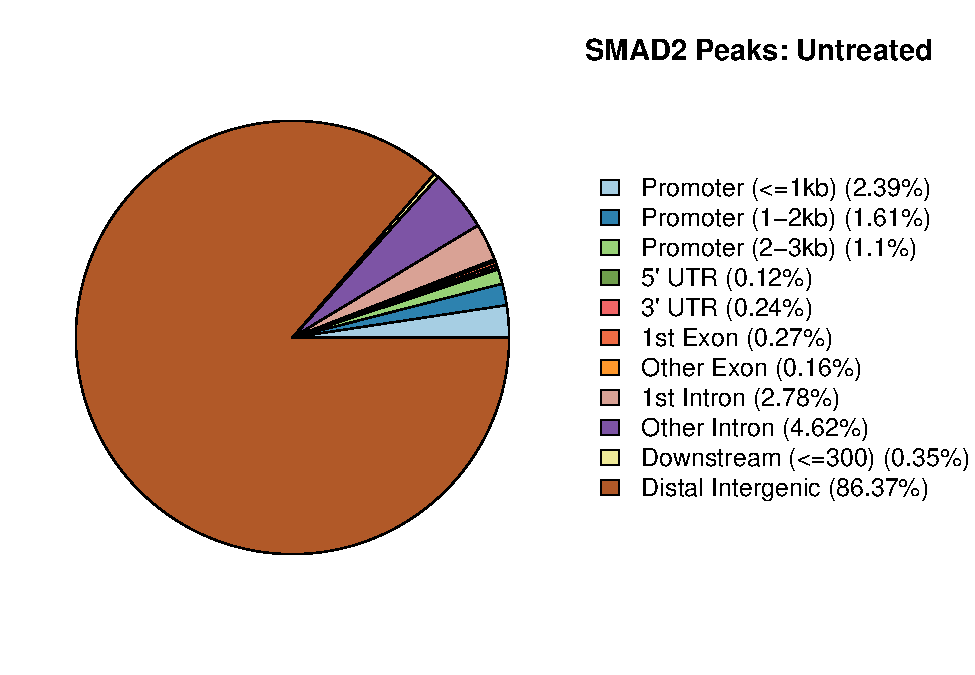
\includegraphics{peak_annotation_go_term_analysis_files/figure-latex/unnamed-chunk-10-1.pdf}

\clearpage{}


\subsubsection{SMAD2 Peaks - Treated}

Similar to the untreated SMAD2 peaks, most of the treated SMAD2 peaks
also lay within the intergenic regions ( about 71\%), but in a lower
proportion as compared to the untreated peaks (about 86\%). On the other
hand, the proportion of SMAD2 peaks in the genic regions rose upon
treatment from 13.28\% to 29.53\%.

\begin{Shaded}
\begin{Highlighting}[]
\KeywordTok{plotAnnoPie}\NormalTok{(AP_SMAD2_abInput_treated_peaks)}
\KeywordTok{title}\NormalTok{(}\DataTypeTok{main =} \StringTok{"SMAD2 Peaks: Treated"}\NormalTok{, }\DataTypeTok{line =} \DecValTok{-2}\NormalTok{, }\DataTypeTok{adj =} \DecValTok{0}\NormalTok{)}
\end{Highlighting}
\end{Shaded}

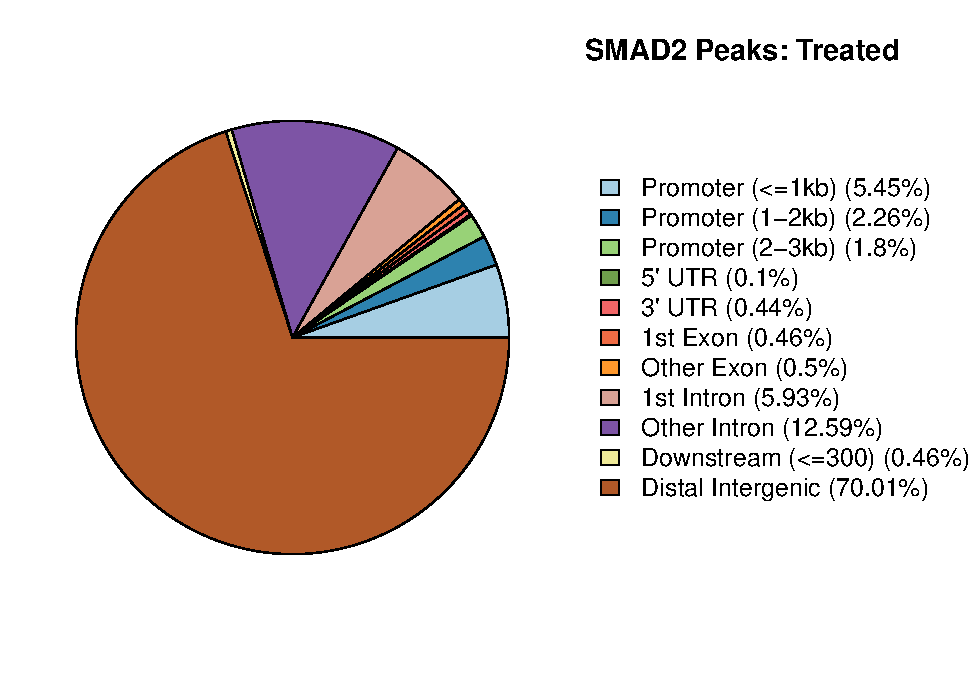
\includegraphics{peak_annotation_go_term_analysis_files/figure-latex/unnamed-chunk-11-1.pdf}

\clearpage{}


\subsubsection{SMAD3 Peaks - Untreated}

Around half of the untreated SMAD3 peaks were in the intergenic regions,
while a majority of the peaks in the genic regions (33.84 \%) overlapped
with intronic sequences. Compared to the SMAD2 peaks (both treated and
untreated), the SMAD3 untreated peaks had a far lower proportion of
peaks within the intergenic regions. On the other hand, the proportion
of SMAD3 peaks in intronic regions was noticeably elevated as compared
to the SMAD2 peaks.

\begin{Shaded}
\begin{Highlighting}[]
\KeywordTok{plotAnnoPie}\NormalTok{(AP_SMAD3_LAP_untreated_peaks)}
\KeywordTok{title}\NormalTok{(}\DataTypeTok{main =} \StringTok{"SMAD3 Peaks: Untreated"}\NormalTok{, }\DataTypeTok{line =} \DecValTok{-2}\NormalTok{, }\DataTypeTok{adj =} \DecValTok{0}\NormalTok{)}
\end{Highlighting}
\end{Shaded}

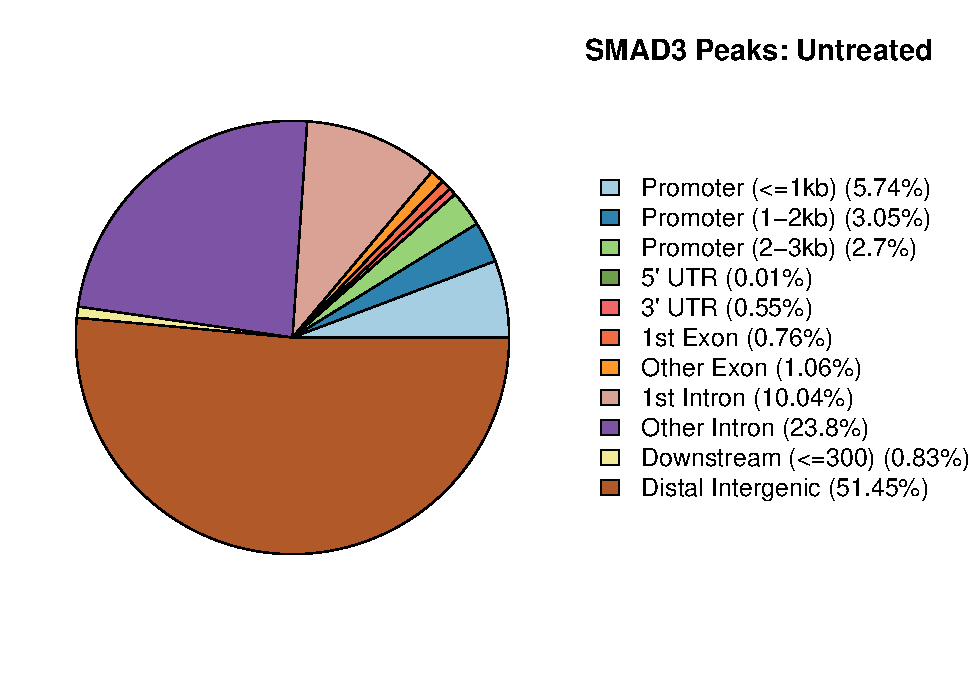
\includegraphics{peak_annotation_go_term_analysis_files/figure-latex/unnamed-chunk-12-1.pdf}

\clearpage{}


\subsubsection{SMAD3 Peaks - Treated}

TGF-\(\beta\) ligand treatment reduced the proportion of SMAD3 peaks in
the intergenic regions (52.28\% without treatment vs.~41.66\% with
treatment). For the most part, those peaks seem to have been displaced
to the promoter regions, which accounted for a total of 11.49\% before
treatment but rose to 18.03\% after treatment.

\begin{Shaded}
\begin{Highlighting}[]
\KeywordTok{plotAnnoPie}\NormalTok{(AP_SMAD3_LAP_treated_peaks)}
\KeywordTok{title}\NormalTok{(}\DataTypeTok{main =} \StringTok{"SMAD3 Peaks: Treated"}\NormalTok{, }\DataTypeTok{line =} \DecValTok{-2}\NormalTok{, }\DataTypeTok{adj =} \DecValTok{0}\NormalTok{)}
\end{Highlighting}
\end{Shaded}

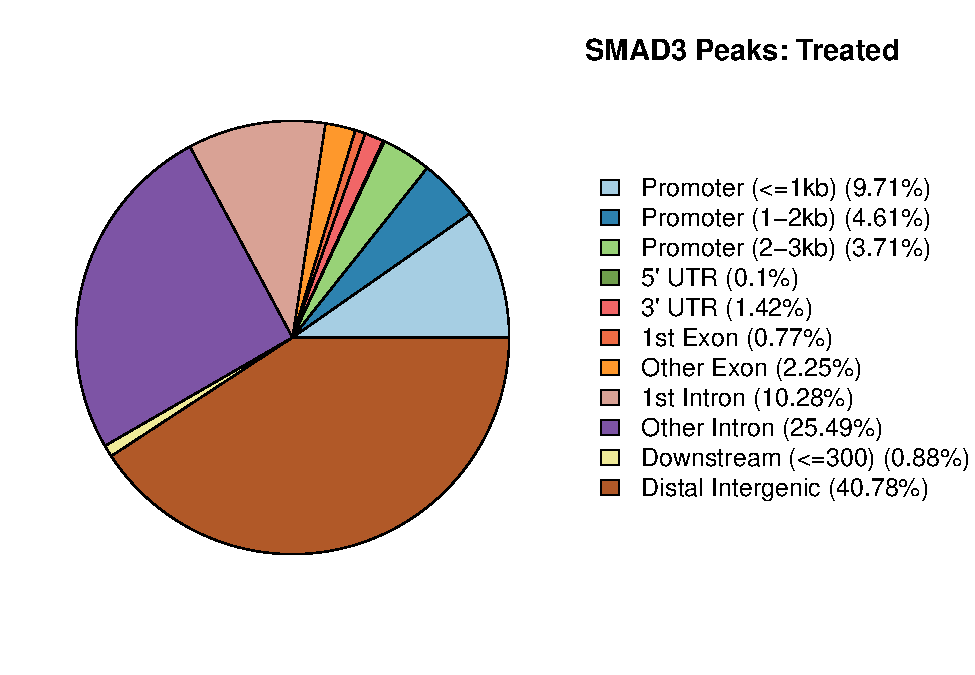
\includegraphics{peak_annotation_go_term_analysis_files/figure-latex/unnamed-chunk-13-1.pdf}

\clearpage{}


\subsection{GO Term Analysis Results}

GO term analysis was limited to biological process (BP) terms; GO Terms
relating to Cellular Component and Molecular Function were not analysed.


\subsubsection{GO Term Analysis for All Peaks}

No enriched BP GO terms were found within annotations for untreated
SMAD2 peaks. This may have been due to the majority of these peaks being
located in the intergenic regions. For treated SMAD2 peaks, GO terms
related to processes in neuronal development were over-represented.

\textbf{Note:} Only the first 20 enriched GO terms for each peak subset
and condition are shown. Terms were arranged in ascending order by
adjusted p value, then in descending order by gene ratio and absolute
count.

\begin{Shaded}
\begin{Highlighting}[]
\NormalTok{ego_SMAD2_abInput_treated_peaks}\OperatorTok{@}\NormalTok{result }\OperatorTok\StringTok{ }
\StringTok{  }\KeywordTok{as_tibble}\NormalTok{() }\OperatorTok\StringTok{ }
\StringTok{  }\KeywordTok{arrange}\NormalTok{(p.adjust, }\KeywordTok{desc}\NormalTok{(Count), }\KeywordTok{desc}\NormalTok{(GeneRatio)) }\OperatorTok\StringTok{ }\KeywordTok{filter}\NormalTok{(p.adjust }\OperatorTok{<}\StringTok{ }\FloatTok{0.05}\NormalTok{) }\OperatorTok\StringTok{  }
\StringTok{  }\NormalTok{dplyr}\OperatorTok{::}\KeywordTok{select}\NormalTok{(Description, p.adjust, GeneRatio, BgRatio) }\OperatorTok\StringTok{ }
\StringTok{  }\KeywordTok{head}\NormalTok{(}\DecValTok{20}\NormalTok{) }\OperatorTok\StringTok{ }
\StringTok{  }\KeywordTok{rename}\NormalTok{(}\DataTypeTok{Description =} \StringTok{"Enriched GO Terms in Treated SMAD2 Peaks"}\NormalTok{) }\OperatorTok\StringTok{ }
\StringTok{  }\KeywordTok{kable}\NormalTok{(}\DataTypeTok{x =}\NormalTok{ ., }\StringTok{"latex"}\NormalTok{, }\DataTypeTok{longtable =}\NormalTok{ T) }\OperatorTok\StringTok{ }\KeywordTok{kable_styling}\NormalTok{(}\DataTypeTok{latex_options =} \KeywordTok{c}\NormalTok{(}\StringTok{"repeat_header"}\NormalTok{))}
\end{Highlighting}
\end{Shaded}

\begin{longtable}{l|r|l|l}
\hline
Enriched GO Terms in Treated SMAD2 Peaks & p.adjust & GeneRatio & BgRatio\\
\hline
\endfirsthead
\multicolumn{4}{@{}l}{\textit{(continued)}}\\
\hline
Enriched GO Terms in Treated SMAD2 Peaks & p.adjust & GeneRatio & BgRatio\\
\hline
\endhead
axon development & 0.0000000 & 80/1342 & 493/18493\\
\hline
axonogenesis & 0.0000001 & 74/1342 & 449/18493\\
\hline
axon guidance & 0.0000002 & 50/1342 & 259/18493\\
\hline
neuron projection guidance & 0.0000002 & 50/1342 & 260/18493\\
\hline
developmental cell growth & 0.0010681 & 38/1342 & 226/18493\\
\hline
developmental growth involved in morphogenesis & 0.0026364 & 37/1342 & 227/18493\\
\hline
neuron projection extension & 0.0035945 & 29/1342 & 161/18493\\
\hline
peptidyl-serine modification & 0.0037980 & 44/1342 & 301/18493\\
\hline
axon extension involved in axon guidance & 0.0037980 & 12/1342 & 37/18493\\
\hline
neuron projection extension involved in neuron projection guidance & 0.0037980 & 12/1342 & 37/18493\\
\hline
regulation of developmental growth & 0.0043011 & 47/1342 & 334/18493\\
\hline
cell junction assembly & 0.0043011 & 37/1342 & 238/18493\\
\hline
regulation of axonogenesis & 0.0066075 & 30/1342 & 180/18493\\
\hline
axon extension & 0.0108430 & 22/1342 & 116/18493\\
\hline
cell growth & 0.0121295 & 60/1342 & 485/18493\\
\hline
peptidyl-serine phosphorylation & 0.0121295 & 40/1342 & 282/18493\\
\hline
regulation of cell morphogenesis involved in differentiation & 0.0125971 & 41/1342 & 293/18493\\
\hline
cell junction organization & 0.0161102 & 40/1342 & 287/18493\\
\hline
smooth muscle contraction & 0.0165590 & 20/1342 & 105/18493\\
\hline
mesenchymal cell development & 0.0165590 & 17/1342 & 82/18493\\
\hline
\end{longtable}

\clearpage{}

\begin{Shaded}
\begin{Highlighting}[]
\KeywordTok{dotplot}\NormalTok{(ego_SMAD2_abInput_treated_peaks) }\OperatorTok{+}\StringTok{ }\KeywordTok{ggtitle}\NormalTok{(}\DataTypeTok{label =} \StringTok{"Enriched BP GO Terms in Treated SMAD2 Peaks"}\NormalTok{) }\OperatorTok{+}\StringTok{ }
\StringTok{    }\KeywordTok{theme}\NormalTok{(}\DataTypeTok{plot.title =} \KeywordTok{element_text}\NormalTok{(}\DataTypeTok{hjust =} \FloatTok{0.8}\NormalTok{, }\DataTypeTok{size =} \DecValTok{15}\NormalTok{), }\DataTypeTok{axis.text.y =} \KeywordTok{element_text}\NormalTok{(}\DataTypeTok{size =} \DecValTok{7}\NormalTok{))}
\end{Highlighting}
\end{Shaded}

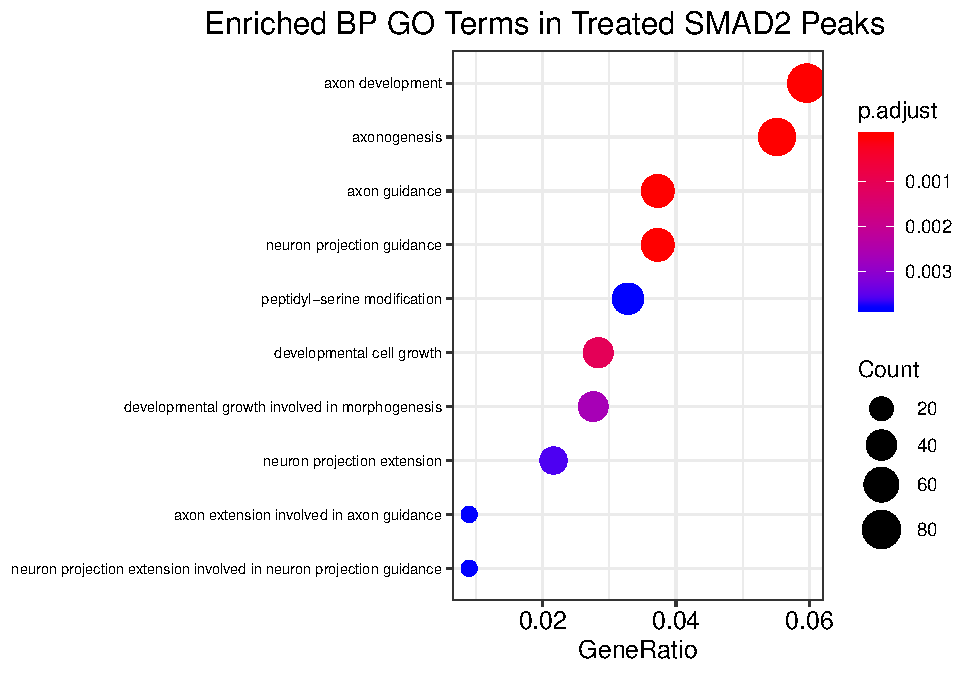
\includegraphics{peak_annotation_go_term_analysis_files/figure-latex/unnamed-chunk-15-1.pdf}

\clearpage{}

Untreated SMAD3 peaks also showed an enrichment in neuronal
development-related terms. In addition, peaks in regions related to
GTPase activity and cell-cell adhesion were also enriched.

\begin{Shaded}
\begin{Highlighting}[]
\NormalTok{ego_SMAD3_LAP_untreated_peaks}\OperatorTok{@}\NormalTok{result }\OperatorTok\StringTok{ }
\StringTok{  }\KeywordTok{as_tibble}\NormalTok{() }\OperatorTok\StringTok{ }
\StringTok{  }\KeywordTok{arrange}\NormalTok{(p.adjust, }\KeywordTok{desc}\NormalTok{(Count) , }\KeywordTok{desc}\NormalTok{(GeneRatio))  }\OperatorTok\StringTok{ }
\StringTok{  }\KeywordTok{filter}\NormalTok{(p.adjust }\OperatorTok{<}\StringTok{ }\FloatTok{0.05}\NormalTok{) }\OperatorTok\StringTok{  }
\StringTok{  }\NormalTok{dplyr}\OperatorTok{::}\KeywordTok{select}\NormalTok{(Description, p.adjust, GeneRatio, BgRatio) }\OperatorTok\StringTok{ }
\StringTok{  }\KeywordTok{head}\NormalTok{(}\DecValTok{20}\NormalTok{) }\OperatorTok\StringTok{ }
\StringTok{  }\KeywordTok{rename}\NormalTok{(}\DataTypeTok{Description =} \StringTok{"Enriched GO Terms in Untreated SMAD3 Peaks"}\NormalTok{) }\OperatorTok\StringTok{ }
\KeywordTok{kable}\NormalTok{( }\DataTypeTok{x =}\NormalTok{ ., }\StringTok{"latex"}\NormalTok{, }\DataTypeTok{longtable =}\NormalTok{ T) }\OperatorTok\StringTok{ }\KeywordTok{kable_styling}\NormalTok{(}\DataTypeTok{latex_options =} \KeywordTok{c}\NormalTok{(}\StringTok{"repeat_header"}\NormalTok{))}
\end{Highlighting}
\end{Shaded}

\begin{longtable}{l|r|l|l}
\hline
Enriched GO Terms in Untreated SMAD3 Peaks & p.adjust & GeneRatio & BgRatio\\
\hline
\endfirsthead
\multicolumn{4}{@{}l}{\textit{(continued)}}\\
\hline
Enriched GO Terms in Untreated SMAD3 Peaks & p.adjust & GeneRatio & BgRatio\\
\hline
\endhead
synapse organization & 0.00e+00 & 138/3612 & 384/18493\\
\hline
cell-cell adhesion via plasma-membrane adhesion molecules & 0.00e+00 & 106/3612 & 270/18493\\
\hline
axon development & 0.00e+00 & 165/3612 & 493/18493\\
\hline
synapse assembly & 0.00e+00 & 73/3612 & 165/18493\\
\hline
axonogenesis & 0.00e+00 & 151/3612 & 449/18493\\
\hline
forebrain development & 1.00e-07 & 125/3612 & 374/18493\\
\hline
homophilic cell adhesion via plasma membrane adhesion molecules & 2.00e-07 & 68/3612 & 167/18493\\
\hline
regulation of neuron projection development & 1.60e-06 & 147/3612 & 478/18493\\
\hline
regulation of GTPase activity & 2.30e-06 & 147/3612 & 481/18493\\
\hline
neuron migration & 7.10e-06 & 59/3612 & 149/18493\\
\hline
positive regulation of GTPase activity & 1.50e-05 & 125/3612 & 405/18493\\
\hline
modulation of chemical synaptic transmission & 1.56e-05 & 128/3612 & 418/18493\\
\hline
regulation of trans-synaptic signaling & 1.69e-05 & 128/3612 & 419/18493\\
\hline
neuron projection guidance & 2.69e-05 & 87/3612 & 260/18493\\
\hline
regulation of synapse organization & 2.69e-05 & 75/3612 & 214/18493\\
\hline
postsynapse organization & 2.69e-05 & 60/3612 & 159/18493\\
\hline
positive regulation of neurogenesis & 2.84e-05 & 135/3612 & 453/18493\\
\hline
regulation of synapse structure or activity & 3.65e-05 & 76/3612 & 220/18493\\
\hline
axon guidance & 3.95e-05 & 86/3612 & 259/18493\\
\hline
regulation of small GTPase mediated signal transduction & 6.12e-05 & 101/3612 & 321/18493\\
\hline
\end{longtable}

\clearpage{}

\begin{Shaded}
\begin{Highlighting}[]
\KeywordTok{dotplot}\NormalTok{(ego_SMAD3_LAP_untreated_peaks) }\OperatorTok{+}\StringTok{ }\KeywordTok{ggtitle}\NormalTok{(}\DataTypeTok{label =} \StringTok{"Enriched BP GO Terms in Untreated SMAD3 Peaks"}\NormalTok{) }\OperatorTok{+}\StringTok{ }\KeywordTok{theme}\NormalTok{(}\DataTypeTok{plot.title =} \KeywordTok{element_text}\NormalTok{(}\DataTypeTok{hjust =} \FloatTok{0.8}\NormalTok{, }\DataTypeTok{size =} \DecValTok{15}\NormalTok{), }\DataTypeTok{axis.text.y =} \KeywordTok{element_text}\NormalTok{(}\DataTypeTok{size =} \DecValTok{7}\NormalTok{))}
\end{Highlighting}
\end{Shaded}

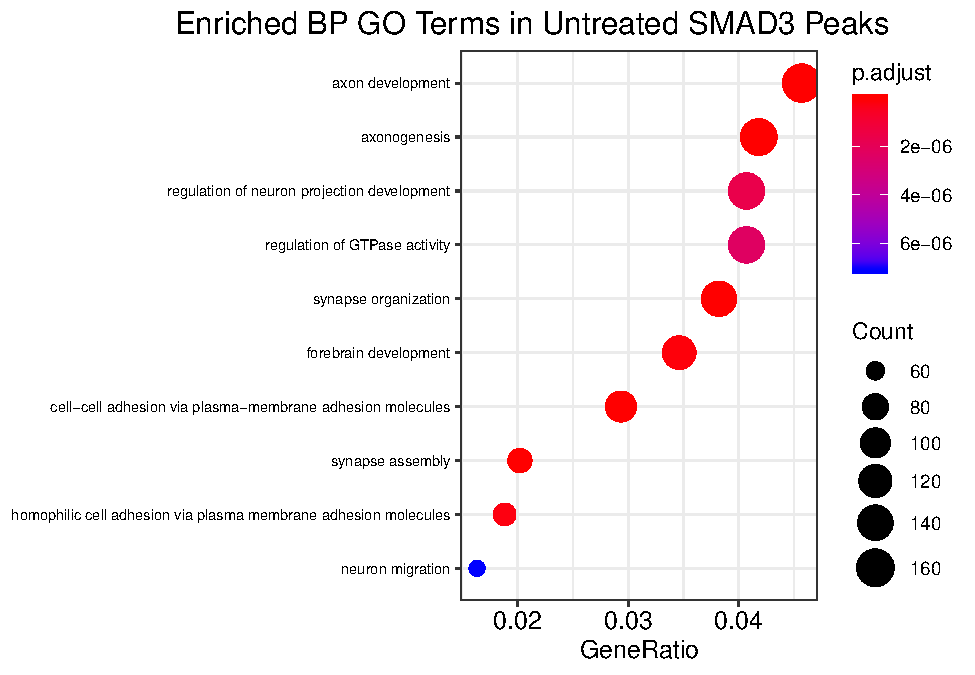
\includegraphics{peak_annotation_go_term_analysis_files/figure-latex/unnamed-chunk-17-1.pdf}

\clearpage{}

Similar terms related to neuronal development also appeared in treated
SMAD3 peaks. However, additional enriched terms such as ``regulation of
small GTPase-mediated signal transduction'', as well as ``regulation of
Ras protein signal transduction'' were also found to be enriched.

\begin{Shaded}
\begin{Highlighting}[]
\NormalTok{ego_SMAD3_LAP_treated_peaks}\OperatorTok{@}\NormalTok{result }\OperatorTok\StringTok{ }
\StringTok{  }\KeywordTok{as_tibble}\NormalTok{() }\OperatorTok\StringTok{ }
\StringTok{  }\KeywordTok{arrange}\NormalTok{(p.adjust, }\KeywordTok{desc}\NormalTok{(Count) , }\KeywordTok{desc}\NormalTok{(GeneRatio))  }\OperatorTok\StringTok{ }
\StringTok{  }\KeywordTok{filter}\NormalTok{(p.adjust }\OperatorTok{<}\StringTok{ }\FloatTok{0.05}\NormalTok{) }\OperatorTok\StringTok{  }
\StringTok{  }\NormalTok{dplyr}\OperatorTok{::}\KeywordTok{select}\NormalTok{(Description, p.adjust, GeneRatio, BgRatio) }\OperatorTok\StringTok{ }
\StringTok{  }\KeywordTok{head}\NormalTok{(}\DecValTok{20}\NormalTok{) }\OperatorTok\StringTok{ }
\StringTok{  }\KeywordTok{rename}\NormalTok{(}\DataTypeTok{Description =} \StringTok{"Enriched GO Terms in Treated SMAD3 Peaks"}\NormalTok{) }\OperatorTok
\StringTok{  }\KeywordTok{kable}\NormalTok{(}\DataTypeTok{x =}\NormalTok{ ., }\StringTok{"latex"}\NormalTok{, }\DataTypeTok{longtable =}\NormalTok{ T) }\OperatorTok\StringTok{ }
\StringTok{  }\KeywordTok{kable_styling}\NormalTok{(}\DataTypeTok{latex_options =} \KeywordTok{c}\NormalTok{(}\StringTok{"repeat_header"}\NormalTok{))}
\end{Highlighting}
\end{Shaded}

\begin{longtable}{l|r|l|l}
\hline
Enriched GO Terms in Treated SMAD3 Peaks & p.adjust & GeneRatio & BgRatio\\
\hline
\endfirsthead
\multicolumn{4}{@{}l}{\textit{(continued)}}\\
\hline
Enriched GO Terms in Treated SMAD3 Peaks & p.adjust & GeneRatio & BgRatio\\
\hline
\endhead
axon development & 0 & 322/8303 & 493/18493\\
\hline
axonogenesis & 0 & 297/8303 & 449/18493\\
\hline
synapse organization & 0 & 253/8303 & 384/18493\\
\hline
regulation of small GTPase mediated signal transduction & 0 & 212/8303 & 321/18493\\
\hline
regulation of GTPase activity & 0 & 297/8303 & 481/18493\\
\hline
positive regulation of GTPase activity & 0 & 254/8303 & 405/18493\\
\hline
regulation of Ras protein signal transduction & 0 & 153/8303 & 222/18493\\
\hline
morphogenesis of an epithelium & 0 & 292/8303 & 479/18493\\
\hline
positive regulation of neurogenesis & 0 & 278/8303 & 453/18493\\
\hline
positive regulation of neuron differentiation & 0 & 226/8303 & 356/18493\\
\hline
synapse assembly & 0 & 119/8303 & 165/18493\\
\hline
neuron projection guidance & 0 & 172/8303 & 260/18493\\
\hline
epithelial tube morphogenesis & 0 & 201/8303 & 313/18493\\
\hline
axon guidance & 0 & 171/8303 & 259/18493\\
\hline
developmental growth involved in morphogenesis & 0 & 153/8303 & 227/18493\\
\hline
regulation of trans-synaptic signaling & 0 & 257/8303 & 419/18493\\
\hline
modulation of chemical synaptic transmission & 0 & 256/8303 & 418/18493\\
\hline
regulation of neuron projection development & 0 & 284/8303 & 478/18493\\
\hline
Ras protein signal transduction & 0 & 259/8303 & 430/18493\\
\hline
positive regulation of cell projection organization & 0 & 227/8303 & 371/18493\\
\hline
\end{longtable}

\clearpage{}

\begin{Shaded}
\begin{Highlighting}[]
\KeywordTok{dotplot}\NormalTok{(ego_SMAD3_LAP_treated_peaks) }\OperatorTok{+}\StringTok{ }\KeywordTok{ggtitle}\NormalTok{(}\DataTypeTok{label =} \StringTok{"Enriched BP GO Terms in Treated SMAD3 Peaks"}\NormalTok{) }\OperatorTok{+}\StringTok{ }\KeywordTok{theme}\NormalTok{(}\DataTypeTok{plot.title =} \KeywordTok{element_text}\NormalTok{(}\DataTypeTok{hjust =} \FloatTok{0.8}\NormalTok{, }\DataTypeTok{size =} \DecValTok{15}\NormalTok{), }\DataTypeTok{axis.text.y =} \KeywordTok{element_text}\NormalTok{(}\DataTypeTok{size =} \DecValTok{7}\NormalTok{))}
\end{Highlighting}
\end{Shaded}

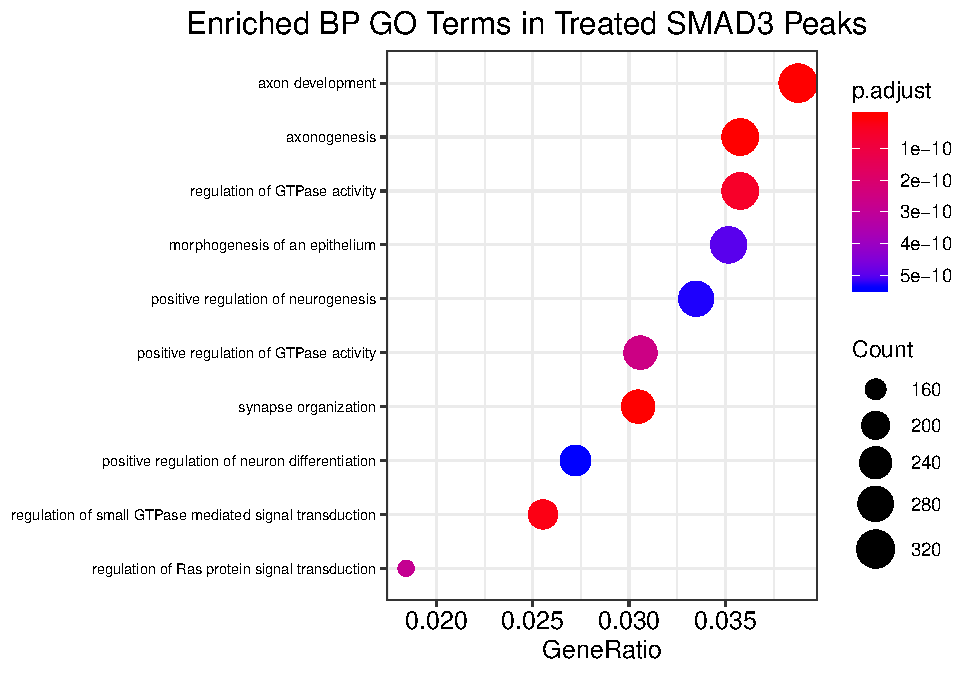
\includegraphics{peak_annotation_go_term_analysis_files/figure-latex/unnamed-chunk-19-1.pdf}

\clearpage{}

\subsubsection{GO Term Analysis for Peaks Restricted to Gene Regions}

The enriched GO Terms for SMAD2 peaks limited to gene regions did not
differ much from their counterparts where all the peaks were considered.
The pattern remains the same, with terms associated with neuronal
development being predominantly featured, although terms for limb and
appendage morphogenesis also turn up.

\begin{Shaded}
\begin{Highlighting}[]
\NormalTok{gen_ego_SMAD2_abInput_treated_peaks}\OperatorTok{@}\NormalTok{result }\OperatorTok\StringTok{ }
\StringTok{  }\KeywordTok{as_tibble}\NormalTok{() }\OperatorTok\StringTok{ }
\StringTok{  }\KeywordTok{arrange}\NormalTok{(p.adjust, }\KeywordTok{desc}\NormalTok{(Count) , }\KeywordTok{desc}\NormalTok{(GeneRatio)) }\OperatorTok\StringTok{ }
\StringTok{  }\KeywordTok{filter}\NormalTok{(p.adjust }\OperatorTok{<}\StringTok{ }\FloatTok{0.05}\NormalTok{) }\OperatorTok\StringTok{  }
\StringTok{  }\NormalTok{dplyr}\OperatorTok{::}\KeywordTok{select}\NormalTok{(Description, p.adjust, GeneRatio, BgRatio) }\OperatorTok\StringTok{ }
\StringTok{  }\KeywordTok{head}\NormalTok{(}\DecValTok{20}\NormalTok{) }\OperatorTok\StringTok{ }
\StringTok{  }\KeywordTok{rename}\NormalTok{(}\DataTypeTok{Description =} \StringTok{"Enriched GO Terms in Treated SMAD2 Peaks Restricted to Gene Regions"}\NormalTok{) }\OperatorTok\StringTok{ }
\StringTok{  }\KeywordTok{kable}\NormalTok{(}\DataTypeTok{x =}\NormalTok{ ., }\StringTok{"latex"}\NormalTok{, }\DataTypeTok{longtable =}\NormalTok{ T) }\OperatorTok\StringTok{ }
\StringTok{  }\KeywordTok{kable_styling}\NormalTok{(}\DataTypeTok{latex_options =} \KeywordTok{c}\NormalTok{(}\StringTok{"repeat_header"}\NormalTok{))}
\end{Highlighting}
\end{Shaded}

\begin{longtable}{l|r|l|l}
\hline
Enriched GO Terms in Treated SMAD2 Peaks Restricted to Gene Regions & p.adjust & GeneRatio & BgRatio\\
\hline
\endfirsthead
\multicolumn{4}{@{}l}{\textit{(continued)}}\\
\hline
Enriched GO Terms in Treated SMAD2 Peaks Restricted to Gene Regions & p.adjust & GeneRatio & BgRatio\\
\hline
\endhead
axonogenesis & 0.0009522 & 46/834 & 449/18493\\
\hline
axon development & 0.0010088 & 48/834 & 493/18493\\
\hline
axon guidance & 0.0010088 & 31/834 & 259/18493\\
\hline
neuron projection guidance & 0.0010088 & 31/834 & 260/18493\\
\hline
synapse organization & 0.0287847 & 36/834 & 384/18493\\
\hline
positive regulation of synaptic transmission, glutamatergic & 0.0433635 & 8/834 & 31/18493\\
\hline
regulation of axonogenesis & 0.0461952 & 21/834 & 180/18493\\
\hline
peptidyl-serine modification & 0.0474595 & 29/834 & 301/18493\\
\hline
positive regulation of synaptic transmission & 0.0474595 & 19/834 & 159/18493\\
\hline
appendage morphogenesis & 0.0474595 & 18/834 & 146/18493\\
\hline
limb morphogenesis & 0.0474595 & 18/834 & 146/18493\\
\hline
\end{longtable}

\clearpage{}

\begin{Shaded}
\begin{Highlighting}[]
\KeywordTok{dotplot}\NormalTok{(gen_ego_SMAD2_abInput_treated_peaks) }\OperatorTok{+}\StringTok{ }\KeywordTok{ggtitle}\NormalTok{(}\DataTypeTok{label =} \StringTok{"Enriched BP GO Terms in Treated SMAD2 Genic Peaks"}\NormalTok{) }\OperatorTok{+}\StringTok{ }\KeywordTok{theme}\NormalTok{(}\DataTypeTok{plot.title =} \KeywordTok{element_text}\NormalTok{(}\DataTypeTok{hjust =} \FloatTok{0.8}\NormalTok{, }\DataTypeTok{size =} \DecValTok{15}\NormalTok{), }\DataTypeTok{axis.text.y =} \KeywordTok{element_text}\NormalTok{(}\DataTypeTok{size =} \DecValTok{7}\NormalTok{))}
\end{Highlighting}
\end{Shaded}

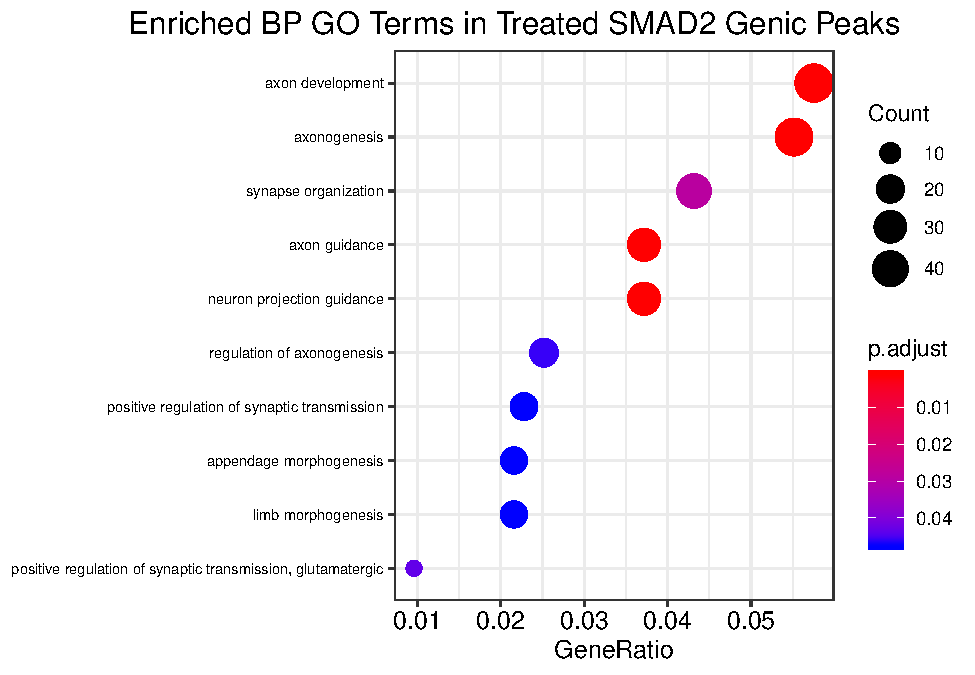
\includegraphics{peak_annotation_go_term_analysis_files/figure-latex/unnamed-chunk-21-1.pdf}

\clearpage{}

Untreated SMAD3 peaks in gene regions showed a similar neuronal
development theme for the most significantly enriched genes.

\begin{Shaded}
\begin{Highlighting}[]
\NormalTok{gen_ego_SMAD3_LAP_untreated_peaks}\OperatorTok{@}\NormalTok{result }\OperatorTok\StringTok{ }
\StringTok{  }\KeywordTok{as_tibble}\NormalTok{() }\OperatorTok\StringTok{ }\KeywordTok{arrange}\NormalTok{(p.adjust, }\KeywordTok{desc}\NormalTok{(Count) , }\KeywordTok{desc}\NormalTok{(GeneRatio))  }\OperatorTok\StringTok{ }
\StringTok{  }\KeywordTok{filter}\NormalTok{(p.adjust }\OperatorTok{<}\StringTok{ }\FloatTok{0.05}\NormalTok{) }\OperatorTok\StringTok{  }
\StringTok{  }\NormalTok{dplyr}\OperatorTok{::}\KeywordTok{select}\NormalTok{(Description, p.adjust, GeneRatio, BgRatio) }\OperatorTok\StringTok{ }
\StringTok{  }\KeywordTok{head}\NormalTok{(}\DecValTok{20}\NormalTok{) }\OperatorTok\StringTok{ }
\StringTok{  }\KeywordTok{rename}\NormalTok{(}\DataTypeTok{Description =} \StringTok{"Enriched GO Terms in Untreated SMAD3 Peaks Restricted to Gene Regions"}\NormalTok{) }\OperatorTok\StringTok{ }
\StringTok{  }\KeywordTok{kable}\NormalTok{(}\DataTypeTok{x =}\NormalTok{ ., }\StringTok{"latex"}\NormalTok{, }\DataTypeTok{longtable =}\NormalTok{ T) }\OperatorTok\StringTok{ }
\StringTok{  }\KeywordTok{kable_styling}\NormalTok{(}\DataTypeTok{latex_options =} \KeywordTok{c}\NormalTok{(}\StringTok{"repeat_header"}\NormalTok{))}
\end{Highlighting}
\end{Shaded}

\begin{longtable}{l|r|l|l}
\hline
Enriched GO Terms in Untreated SMAD3 Peaks Restricted to Gene Regions & p.adjust & GeneRatio & BgRatio\\
\hline
\endfirsthead
\multicolumn{4}{@{}l}{\textit{(continued)}}\\
\hline
Enriched GO Terms in Untreated SMAD3 Peaks Restricted to Gene Regions & p.adjust & GeneRatio & BgRatio\\
\hline
\endhead
axonogenesis & 0.00e+00 & 118/2341 & 449/18493\\
\hline
axon development & 0.00e+00 & 124/2341 & 493/18493\\
\hline
cell-cell adhesion via plasma-membrane adhesion molecules & 0.00e+00 & 80/2341 & 270/18493\\
\hline
homophilic cell adhesion via plasma membrane adhesion molecules & 0.00e+00 & 55/2341 & 167/18493\\
\hline
regulation of neuron projection development & 0.00e+00 & 113/2341 & 478/18493\\
\hline
synapse organization & 0.00e+00 & 96/2341 & 384/18493\\
\hline
synapse assembly & 5.00e-07 & 51/2341 & 165/18493\\
\hline
neuron projection guidance & 7.00e-07 & 69/2341 & 260/18493\\
\hline
axon guidance & 1.40e-06 & 68/2341 & 259/18493\\
\hline
regulation of GTPase activity & 1.50e-06 & 107/2341 & 481/18493\\
\hline
modulation of chemical synaptic transmission & 1.60e-06 & 96/2341 & 418/18493\\
\hline
regulation of trans-synaptic signaling & 1.70e-06 & 96/2341 & 419/18493\\
\hline
neuron migration & 1.80e-06 & 46/2341 & 149/18493\\
\hline
positive regulation of GTPase activity & 4.80e-06 & 92/2341 & 405/18493\\
\hline
positive regulation of neurogenesis & 5.00e-06 & 100/2341 & 453/18493\\
\hline
forebrain development & 1.39e-05 & 85/2341 & 374/18493\\
\hline
sensory system development & 1.39e-05 & 82/2341 & 357/18493\\
\hline
eye development & 1.39e-05 & 81/2341 & 351/18493\\
\hline
visual system development & 1.46e-05 & 81/2341 & 352/18493\\
\hline
positive regulation of neuron differentiation & 2.32e-05 & 81/2341 & 356/18493\\
\hline
\end{longtable}

\clearpage{}

\begin{Shaded}
\begin{Highlighting}[]
\KeywordTok{dotplot}\NormalTok{(gen_ego_SMAD3_LAP_untreated_peaks ) }\OperatorTok{+}\StringTok{ }\KeywordTok{ggtitle}\NormalTok{(}\DataTypeTok{label =} \StringTok{"Enriched BP GO Terms in Untreated SMAD3 Genic Peaks"}\NormalTok{) }\OperatorTok{+}\StringTok{ }\KeywordTok{theme}\NormalTok{(}\DataTypeTok{plot.title =} \KeywordTok{element_text}\NormalTok{(}\DataTypeTok{hjust =} \FloatTok{0.8}\NormalTok{, }\DataTypeTok{size =} \DecValTok{15}\NormalTok{), }\DataTypeTok{axis.text.y =} \KeywordTok{element_text}\NormalTok{(}\DataTypeTok{size =} \DecValTok{7}\NormalTok{))}
\end{Highlighting}
\end{Shaded}

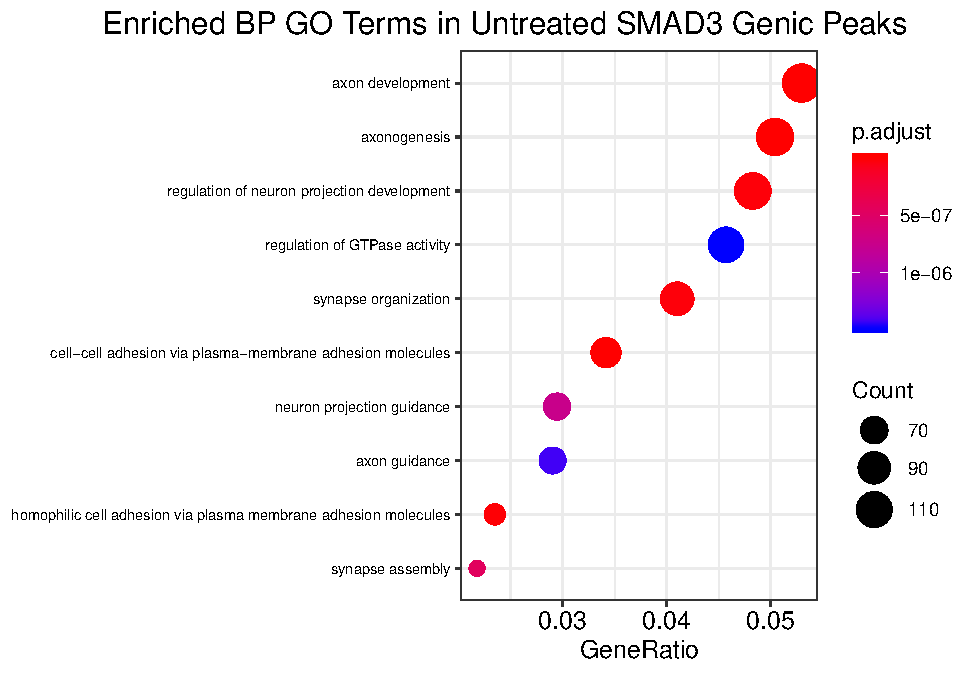
\includegraphics{peak_annotation_go_term_analysis_files/figure-latex/unnamed-chunk-23-1.pdf}

\clearpage{}

Treated SMAD3 peaks in gene regions did not show too many chages either,
as compared to the the set of all treated SMAD3 peaks.

\begin{Shaded}
\begin{Highlighting}[]
\KeywordTok{kable}\NormalTok{(gen_ego_SMAD3_LAP_treated_peaks}\OperatorTok{@}\NormalTok{result }\OperatorTok\StringTok{ }\KeywordTok{as_tibble}\NormalTok{() }\OperatorTok\StringTok{ }\KeywordTok{arrange}\NormalTok{(p.adjust, }\KeywordTok{desc}\NormalTok{(Count) , }\KeywordTok{desc}\NormalTok{(GeneRatio))  }\OperatorTok\StringTok{ }\KeywordTok{filter}\NormalTok{(p.adjust }\OperatorTok{<}\StringTok{ }\FloatTok{0.05}\NormalTok{) }\OperatorTok\StringTok{  }\NormalTok{dplyr}\OperatorTok{::}\KeywordTok{select}\NormalTok{(Description, p.adjust, GeneRatio, BgRatio) }\OperatorTok\StringTok{ }\KeywordTok{head}\NormalTok{(}\DecValTok{20}\NormalTok{) }\OperatorTok\StringTok{ }\KeywordTok{rename}\NormalTok{(}\DataTypeTok{Description =} \StringTok{"Enriched GO Terms in Treated SMAD3 Peaks Restricted to Gene Regions"}\NormalTok{), }\StringTok{"latex"}\NormalTok{, }\DataTypeTok{longtable =}\NormalTok{ T) }\OperatorTok\StringTok{ }\KeywordTok{kable_styling}\NormalTok{(}\DataTypeTok{latex_options =} \KeywordTok{c}\NormalTok{(}\StringTok{"repeat_header"}\NormalTok{))}
\end{Highlighting}
\end{Shaded}

\begin{longtable}{l|r|l|l}
\hline
Enriched GO Terms in Treated SMAD3 Peaks Restricted to Gene Regions & p.adjust & GeneRatio & BgRatio\\
\hline
\endfirsthead
\multicolumn{4}{@{}l}{\textit{(continued)}}\\
\hline
Enriched GO Terms in Treated SMAD3 Peaks Restricted to Gene Regions & p.adjust & GeneRatio & BgRatio\\
\hline
\endhead
axon development & 0 & 273/6456 & 493/18493\\
\hline
axonogenesis & 0 & 253/6456 & 449/18493\\
\hline
regulation of GTPase activity & 0 & 258/6456 & 481/18493\\
\hline
synapse organization & 0 & 215/6456 & 384/18493\\
\hline
positive regulation of neuron differentiation & 0 & 199/6456 & 356/18493\\
\hline
positive regulation of neurogenesis & 0 & 239/6456 & 453/18493\\
\hline
positive regulation of GTPase activity & 0 & 217/6456 & 405/18493\\
\hline
positive regulation of cell projection organization & 0 & 201/6456 & 371/18493\\
\hline
regulation of small GTPase mediated signal transduction & 0 & 177/6456 & 321/18493\\
\hline
regulation of neuron projection development & 0 & 245/6456 & 478/18493\\
\hline
regulation of Ras protein signal transduction & 0 & 130/6456 & 222/18493\\
\hline
regulation of axonogenesis & 0 & 110/6456 & 180/18493\\
\hline
neuron projection guidance & 0 & 147/6456 & 260/18493\\
\hline
axon guidance & 0 & 146/6456 & 259/18493\\
\hline
modulation of chemical synaptic transmission & 0 & 213/6456 & 418/18493\\
\hline
regulation of trans-synaptic signaling & 0 & 213/6456 & 419/18493\\
\hline
positive regulation of neuron projection development & 0 & 147/6456 & 269/18493\\
\hline
developmental growth involved in morphogenesis & 0 & 128/6456 & 227/18493\\
\hline
regulation of cell morphogenesis involved in differentiation & 0 & 157/6456 & 293/18493\\
\hline
synapse assembly & 0 & 99/6456 & 165/18493\\
\hline
\end{longtable}

\clearpage{}

\begin{Shaded}
\begin{Highlighting}[]
\KeywordTok{dotplot}\NormalTok{(gen_ego_SMAD3_LAP_treated_peaks )}\OperatorTok{+}\StringTok{ }\KeywordTok{ggtitle}\NormalTok{(}\DataTypeTok{label =} \StringTok{"Enriched BP GO Terms in Treated SMAD3 Genic Peaks"}\NormalTok{) }\OperatorTok{+}\StringTok{ }\KeywordTok{theme}\NormalTok{(}\DataTypeTok{plot.title =} \KeywordTok{element_text}\NormalTok{(}\DataTypeTok{hjust =} \FloatTok{0.8}\NormalTok{, }\DataTypeTok{size =} \DecValTok{15}\NormalTok{), }\DataTypeTok{axis.text.y =} \KeywordTok{element_text}\NormalTok{(}\DataTypeTok{size =} \DecValTok{7}\NormalTok{))}
\end{Highlighting}
\end{Shaded}

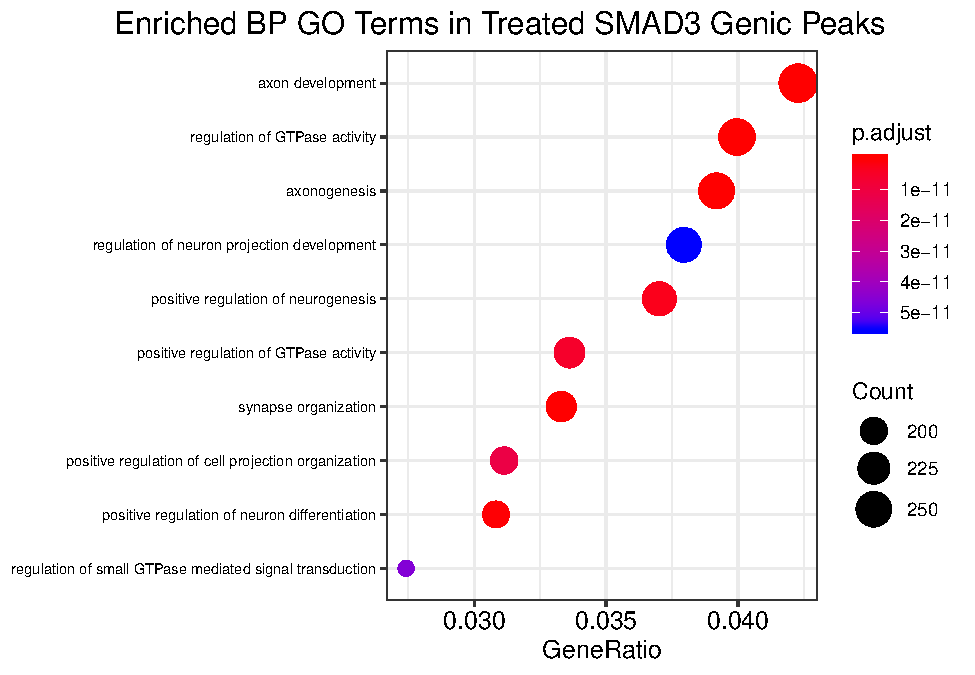
\includegraphics{peak_annotation_go_term_analysis_files/figure-latex/unnamed-chunk-25-1.pdf}

\clearpage{}


\subsubsection{GO Term Analysis for Peaks Restricted to Promoter Regions}

When peaks were limited to promoter regions, the enriched GO term sets
showed noticeable differences from sets derived from all peaks as well
as sets derived from peaks limited to gene regions. No enriched GO terms
were found for treated promoter-proximal SMAD2 peaks.

\begin{Shaded}
\begin{Highlighting}[]
\NormalTok{prom_ego_SMAD2_abInput_untreated_peaks}\OperatorTok{@}\NormalTok{result }\OperatorTok\StringTok{ }
\StringTok{  }\KeywordTok{as_tibble}\NormalTok{() }\OperatorTok\StringTok{ }
\StringTok{  }\KeywordTok{arrange}\NormalTok{(p.adjust, }\KeywordTok{desc}\NormalTok{(Count) , }\KeywordTok{desc}\NormalTok{(GeneRatio))  }\OperatorTok\StringTok{ }
\StringTok{  }\KeywordTok{filter}\NormalTok{(p.adjust }\OperatorTok{<}\StringTok{ }\FloatTok{0.05}\NormalTok{) }\OperatorTok\StringTok{  }
\StringTok{  }\NormalTok{dplyr}\OperatorTok{::}\KeywordTok{select}\NormalTok{(Description, p.adjust, GeneRatio, BgRatio) }\OperatorTok\StringTok{ }
\StringTok{  }\KeywordTok{head}\NormalTok{(}\DecValTok{20}\NormalTok{) }\OperatorTok\StringTok{ }
\StringTok{  }\KeywordTok{rename}\NormalTok{(}\DataTypeTok{Description =} \StringTok{"Enriched GO Terms in Untreated SMAD2 Peaks Restricted to Promoters"}\NormalTok{) }\OperatorTok\StringTok{ }
\StringTok{  }\KeywordTok{kable}\NormalTok{(}\DataTypeTok{x =}\NormalTok{ ., }\StringTok{"latex"}\NormalTok{, }\DataTypeTok{longtable =}\NormalTok{ T) }\OperatorTok\StringTok{ }
\StringTok{  }\KeywordTok{kable_styling}\NormalTok{(}\DataTypeTok{latex_options =} \KeywordTok{c}\NormalTok{(}\StringTok{"repeat_header"}\NormalTok{))}
\end{Highlighting}
\end{Shaded}

\begin{longtable}{l|r|l|l}
\hline
Enriched GO Terms in Untreated SMAD2 Peaks Restricted to Promoters & p.adjust & GeneRatio & BgRatio\\
\hline
\endfirsthead
\multicolumn{4}{@{}l}{\textit{(continued)}}\\
\hline
Enriched GO Terms in Untreated SMAD2 Peaks Restricted to Promoters & p.adjust & GeneRatio & BgRatio\\
\hline
\endhead
negative regulation of execution phase of apoptosis & 0.0190118 & 3/43 & 23/18493\\
\hline
extracellular regulation of signal transduction & 0.0220964 & 3/43 & 36/18493\\
\hline
extracellular negative regulation of signal transduction & 0.0220964 & 3/43 & 36/18493\\
\hline
regulation of execution phase of apoptosis & 0.0220964 & 3/43 & 38/18493\\
\hline
pyrimidine nucleotide biosynthetic process & 0.0356605 & 3/43 & 48/18493\\
\hline
signal transduction in response to DNA damage & 0.0367235 & 4/43 & 130/18493\\
\hline
blood vessel endothelial cell differentiation & 0.0387759 & 2/43 & 11/18493\\
\hline
pyrimidine-containing compound biosynthetic process & 0.0391230 & 3/43 & 58/18493\\
\hline
pyrimidine nucleotide metabolic process & 0.0396258 & 3/43 & 64/18493\\
\hline
CDP-diacylglycerol biosynthetic process & 0.0396258 & 2/43 & 13/18493\\
\hline
CDP-diacylglycerol metabolic process & 0.0396258 & 2/43 & 14/18493\\
\hline
morphogenesis of an endothelium & 0.0396258 & 2/43 & 15/18493\\
\hline
endothelial tube morphogenesis & 0.0396258 & 2/43 & 15/18493\\
\hline
\end{longtable}

\clearpage{}

\begin{Shaded}
\begin{Highlighting}[]
\KeywordTok{dotplot}\NormalTok{(prom_ego_SMAD2_abInput_untreated_peaks) }\OperatorTok{+}\StringTok{ }\KeywordTok{ggtitle}\NormalTok{(}\DataTypeTok{label =} \StringTok{"Enriched BP GO Terms in Untreated SMAD2 Promoter Peaks"}\NormalTok{) }\OperatorTok{+}\StringTok{ }\KeywordTok{theme}\NormalTok{(}\DataTypeTok{plot.title =} \KeywordTok{element_text}\NormalTok{(}\DataTypeTok{hjust =} \FloatTok{0.8}\NormalTok{, }\DataTypeTok{size =} \DecValTok{15}\NormalTok{), }\DataTypeTok{axis.text.y =} \KeywordTok{element_text}\NormalTok{(}\DataTypeTok{size =} \DecValTok{7}\NormalTok{))}
\end{Highlighting}
\end{Shaded}

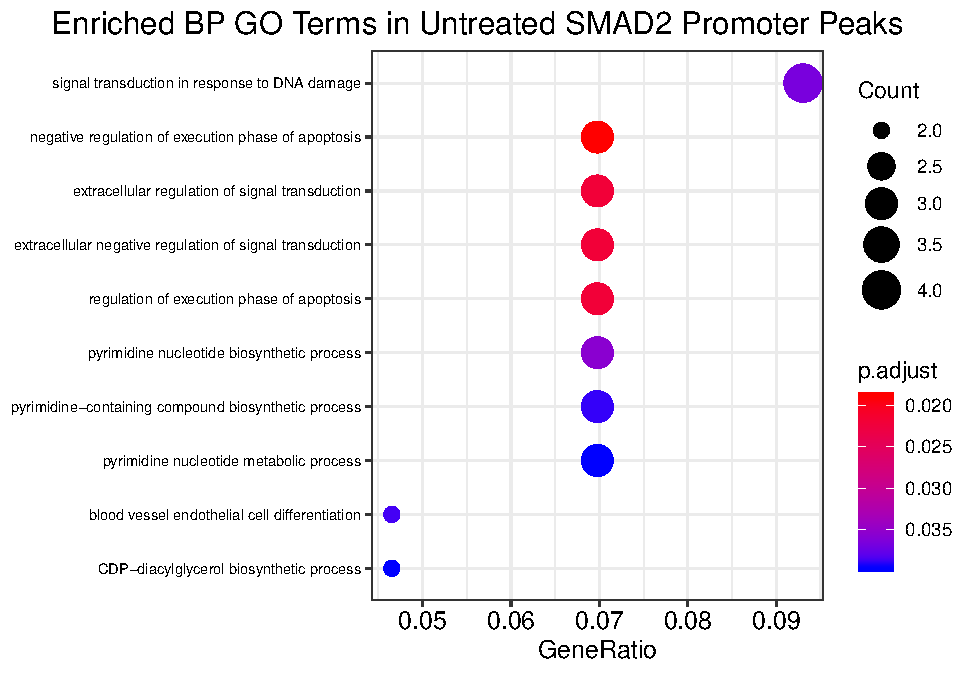
\includegraphics{peak_annotation_go_term_analysis_files/figure-latex/unnamed-chunk-27-1.pdf}

\clearpage{}

Untreated SMAD3 peaks restricted to promoters showed the least number of
enriched terms, all of which were related to cell-cell adhesion.

\begin{Shaded}
\begin{Highlighting}[]
\NormalTok{prom_ego_SMAD3_LAP_untreated_peaks}\OperatorTok{@}\NormalTok{result }\OperatorTok\StringTok{ }
\StringTok{  }\KeywordTok{as_tibble}\NormalTok{() }\OperatorTok\StringTok{ }
\StringTok{  }\KeywordTok{arrange}\NormalTok{(p.adjust, }\KeywordTok{desc}\NormalTok{(Count) , }\KeywordTok{desc}\NormalTok{(GeneRatio))  }\OperatorTok\StringTok{ }
\StringTok{  }\KeywordTok{filter}\NormalTok{(p.adjust }\OperatorTok{<}\StringTok{ }\FloatTok{0.05}\NormalTok{) }\OperatorTok\StringTok{  }
\StringTok{  }\NormalTok{dplyr}\OperatorTok{::}\KeywordTok{select}\NormalTok{(Description, p.adjust, GeneRatio, BgRatio) }\OperatorTok\StringTok{ }
\StringTok{  }\KeywordTok{head}\NormalTok{(}\DecValTok{20}\NormalTok{) }\OperatorTok\StringTok{ }
\StringTok{  }\KeywordTok{rename}\NormalTok{(}\DataTypeTok{Description =} \StringTok{"Enriched GO Terms in Untreated SMAD3 Peaks Restricted to Promoters"}\NormalTok{) }\OperatorTok\StringTok{ }
\StringTok{  }\KeywordTok{kable}\NormalTok{(}\DataTypeTok{x =}\NormalTok{ . , }\StringTok{"latex"}\NormalTok{, }\DataTypeTok{longtable =}\NormalTok{ T) }\OperatorTok\StringTok{ }\KeywordTok{kable_styling}\NormalTok{(}\DataTypeTok{latex_options =} \KeywordTok{c}\NormalTok{(}\StringTok{"repeat_header"}\NormalTok{))}
\end{Highlighting}
\end{Shaded}

\begin{longtable}{l|r|l|l}
\hline
Enriched GO Terms in Untreated SMAD3 Peaks Restricted to Promoters & p.adjust & GeneRatio & BgRatio\\
\hline
\endfirsthead
\multicolumn{4}{@{}l}{\textit{(continued)}}\\
\hline
Enriched GO Terms in Untreated SMAD3 Peaks Restricted to Promoters & p.adjust & GeneRatio & BgRatio\\
\hline
\endhead
homophilic cell adhesion via plasma membrane adhesion molecules & 0.0000000 & 29/655 & 167/18493\\
\hline
cell-cell adhesion via plasma-membrane adhesion molecules & 0.0000194 & 31/655 & 270/18493\\
\hline
calcium-dependent cell-cell adhesion via plasma membrane cell adhesion molecules & 0.0001125 & 12/655 & 48/18493\\
\hline
\end{longtable}

\clearpage{}

\begin{Shaded}
\begin{Highlighting}[]
\KeywordTok{dotplot}\NormalTok{(prom_ego_SMAD3_LAP_untreated_peaks) }\OperatorTok{+}\StringTok{ }\KeywordTok{ggtitle}\NormalTok{(}\DataTypeTok{label =} \StringTok{"Enriched BP GO Terms in Untreated SMAD3 Promoter Peaks"}\NormalTok{) }\OperatorTok{+}\StringTok{ }\KeywordTok{theme}\NormalTok{(}\DataTypeTok{plot.title =} \KeywordTok{element_text}\NormalTok{(}\DataTypeTok{hjust =} \FloatTok{0.8}\NormalTok{, }\DataTypeTok{size =} \DecValTok{15}\NormalTok{), }\DataTypeTok{axis.text.y =} \KeywordTok{element_text}\NormalTok{(}\DataTypeTok{size =} \DecValTok{7}\NormalTok{))}
\end{Highlighting}
\end{Shaded}

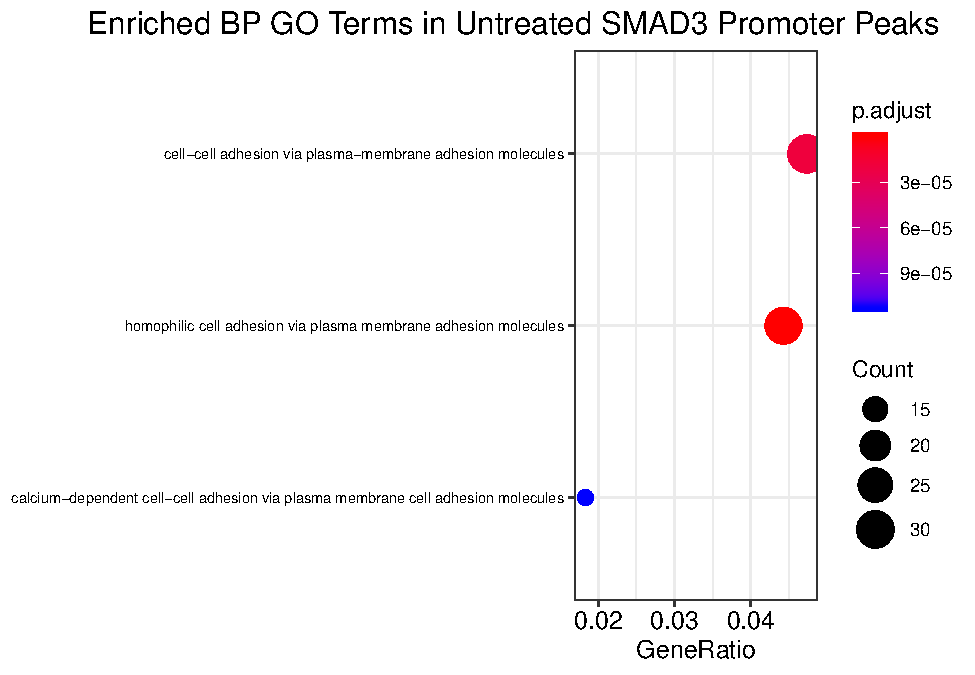
\includegraphics{peak_annotation_go_term_analysis_files/figure-latex/unnamed-chunk-29-1.pdf}

\clearpage{}

Treatment with ligand seemed to show many more enriched GO terms in
promoter-restricted SMAD3 peaks, as compared to untreated
promoter-restricted SMAD3 peaks.

\begin{Shaded}
\begin{Highlighting}[]
\NormalTok{prom_ego_SMAD3_LAP_treated_peaks}\OperatorTok{@}\NormalTok{result }\OperatorTok\StringTok{ }
\StringTok{  }\KeywordTok{as_tibble}\NormalTok{() }\OperatorTok\StringTok{ }
\StringTok{  }\KeywordTok{arrange}\NormalTok{(p.adjust, }\KeywordTok{desc}\NormalTok{(Count) , }\KeywordTok{desc}\NormalTok{(GeneRatio))  }\OperatorTok\StringTok{ }
\StringTok{  }\KeywordTok{filter}\NormalTok{(p.adjust }\OperatorTok{<}\StringTok{ }\FloatTok{0.05}\NormalTok{) }\OperatorTok\StringTok{  }
\StringTok{  }\NormalTok{dplyr}\OperatorTok{::}\KeywordTok{select}\NormalTok{(Description, p.adjust, GeneRatio, BgRatio) }\OperatorTok\StringTok{ }
\StringTok{  }\KeywordTok{head}\NormalTok{(}\DecValTok{20}\NormalTok{) }\OperatorTok
\StringTok{  }\KeywordTok{rename}\NormalTok{(}\DataTypeTok{Description =} \StringTok{"Enriched GO Terms in Treated SMAD3 Peaks Restricted to Promoters"}\NormalTok{) }\OperatorTok\StringTok{ }
\StringTok{  }\KeywordTok{kable}\NormalTok{(}\DataTypeTok{x =}\NormalTok{ . , }\StringTok{"latex"}\NormalTok{, }\DataTypeTok{longtable =}\NormalTok{ T) }\OperatorTok\StringTok{ }
\StringTok{  }\KeywordTok{kable_styling}\NormalTok{(}\DataTypeTok{latex_options =} \KeywordTok{c}\NormalTok{(}\StringTok{"repeat_header"}\NormalTok{))}
\end{Highlighting}
\end{Shaded}

\begin{longtable}{l|r|l|l}
\hline
Enriched GO Terms in Treated SMAD3 Peaks Restricted to Promoters & p.adjust & GeneRatio & BgRatio\\
\hline
\endfirsthead
\multicolumn{4}{@{}l}{\textit{(continued)}}\\
\hline
Enriched GO Terms in Treated SMAD3 Peaks Restricted to Promoters & p.adjust & GeneRatio & BgRatio\\
\hline
\endhead
regulation of small GTPase mediated signal transduction & 0.0000001 & 99/2990 & 321/18493\\
\hline
regulation of Ras protein signal transduction & 0.0000001 & 76/2990 & 222/18493\\
\hline
regulation of GTPase activity & 0.0000017 & 129/2990 & 481/18493\\
\hline
positive regulation of GTPase activity & 0.0000017 & 113/2990 & 405/18493\\
\hline
regulation of Rho protein signal transduction & 0.0000017 & 51/2990 & 136/18493\\
\hline
Rho protein signal transduction & 0.0002438 & 61/2990 & 199/18493\\
\hline
activation of GTPase activity & 0.0007166 & 34/2990 & 91/18493\\
\hline
Ras protein signal transduction & 0.0013685 & 107/2990 & 430/18493\\
\hline
epithelial tube morphogenesis & 0.0045268 & 81/2990 & 313/18493\\
\hline
extracellular matrix organization & 0.0230640 & 85/2990 & 348/18493\\
\hline
pinocytosis & 0.0230640 & 11/2990 & 19/18493\\
\hline
morphogenesis of an epithelium & 0.0276288 & 110/2990 & 479/18493\\
\hline
extracellular structure organization & 0.0276288 & 95/2990 & 402/18493\\
\hline
regulation of phosphoprotein phosphatase activity & 0.0349439 & 35/2990 & 114/18493\\
\hline
endosomal transport & 0.0392397 & 55/2990 & 208/18493\\
\hline
neural tube closure & 0.0392397 & 29/2990 & 89/18493\\
\hline
tube closure & 0.0401784 & 29/2990 & 90/18493\\
\hline
histone H3-K36 methylation & 0.0401784 & 8/2990 & 12/18493\\
\hline
distal tubule development & 0.0401784 & 8/2990 & 12/18493\\
\hline
tube formation & 0.0492196 & 41/2990 & 145/18493\\
\hline
\end{longtable}

\clearpage{}

\begin{Shaded}
\begin{Highlighting}[]
\KeywordTok{dotplot}\NormalTok{(prom_ego_SMAD3_LAP_treated_peaks) }\OperatorTok{+}\StringTok{ }\KeywordTok{ggtitle}\NormalTok{(}\DataTypeTok{label =} \StringTok{"Enriched BP GO Term in Treated SMAD3 Promoter Peaks"}\NormalTok{) }\OperatorTok{+}\StringTok{ }\KeywordTok{theme}\NormalTok{(}\DataTypeTok{plot.title =} \KeywordTok{element_text}\NormalTok{(}\DataTypeTok{hjust =} \FloatTok{0.8}\NormalTok{, }\DataTypeTok{size =} \DecValTok{15}\NormalTok{), }\DataTypeTok{axis.text.y =} \KeywordTok{element_text}\NormalTok{(}\DataTypeTok{size =} \DecValTok{7}\NormalTok{))}
\end{Highlighting}
\end{Shaded}

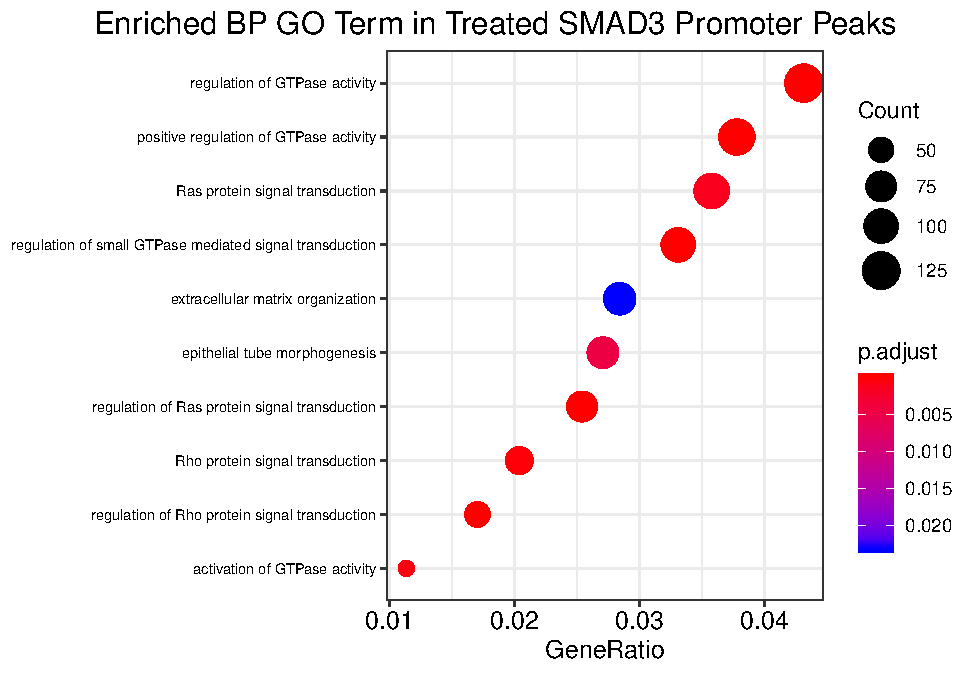
\includegraphics{peak_annotation_go_term_analysis_files/figure-latex/unnamed-chunk-31-1.pdf}


\end{document}
